%%%%%%%%%%%%%%%%%%%%%%%%%%%%%%%%%
% 6CCS3PRJ Final Year Individual Project Report
% mohammad.i.khan@kcl.ac.uk
%%%%%%%%%%%%%%%%%%%%%%%%%%%%%%%%%
\documentclass[20pt]{informatics-report}
\setlength{\parskip}{1em}
\usepackage{color}
\usepackage{caption}
\usepackage{pgfplots}
\usepackage{graphicx}
\usepackage{booktabs}
\usepackage{amsmath}
\usepackage{subcaption}
\usepackage{algorithm}
\usepackage{url}
\usepackage{algpseudocode}
\usepackage[square,sort,comma,numbers]{natbib} %References

%%%%%%%%%%%%%%%%%%%%%%%%%%%%%%%%%
% Front Matter - project title, name, supervisor name and date
%%%%%%%%%%%%%%%%%%%%%%%%%%%%%%%%%
% \title{6CCS3PRJ Final Year\\\vspace{0.2cm}Individual Project Report Title}
\title{Naive Bayes Classifier in a Chess Engine}
\author{Mohammad Ibrahim Khan}
\studentID{k22013981}
\supervisor{Jeffery Raphael}



\date{\today}

\abstractFile{FrontMatter/abstract.tex}
% \ackFile{FrontMatter/acknowledgements.tex} %Remove line if you do not want acknowledgements

\begin{document}
\createFrontMatter
\onehalfspacing
\tableofcontents
\doublespacing

%%%%%%%%%%%%%%%%%%%%%%%%%%%%%%%%%
% Report Content
%%%%%%%%%%%%%%%%%%%%%%%%%%%%%%%%%
% You can write each chapter directly here or in a separate .tex file and use the include command.

\chapter{Introduction}


Since the creation of chess over 1500 years ago \cite{davidsonShortHistoryChess2012}, it is widely acknowledged among researchers and players that the most influential moment in chess history was IBM's Deep Blue defeating Kasparov \cite{hsuIBMsDeepBlue1999}, the world champion at the time. This was a turning point for chess engines and AI in general.
Since then we have seen the rise of more complex and powerful chess engines the likes of Stockfish and AlphaZero. Despite our progress in this field, the game is still unsolved, not being able to definitively determine the best move in a given position. Shannon (1950) mentions that there are $10^{120}$ possible positions in chess \cite{shannonXXIIProgrammingComputer1950} which is more than the number of atoms in the universe. Therefore, brute-forcing the game remains infeasible. As a result, since 1997, attempts have been made to create a perfect chess engine. Achieving more efficient approaches to solving chess could provide meaningful insights into other problems in computer science like optimisation and decision-making.

Machine Learning is at the heart of modern chess engines like AlphaZero and Stockfish.  
% ??MENTION WHAT IS USED BY STOCKFISH OR ALPHAZERO AND QUOTE???. 
This project aims to create a chess engine that uses machine learning techniques that are not popular within chess engines, to explore the potential of these techniques and their effectiveness. Chess engines are usually used as a benchmark for advancements in AI, so this project could be a stepping stone for future research. 

Minimax, especially when combined with Alpha-Beta pruning, is fundamental to modern chess engines. Alpha-Beta pruning optimises the algorithm by discarding unnecessary branches within a game tree which decreases the computational demand considerably. Despite this, even optimised minimax algorithms cannot fully explore an entire tree due to exponential growth. This is where machine learning is used to predict optimal moves more efficiently. Many techniques have been used from Neural Networks \cite{kleinNeuralNetworksChess2022} to Natural Language Processing (NLP) \cite{NLPinChess}. 

This research focuses on how a Naive Bayes Classifier can be implemented in a search algorithm like Minimax to improve positional evaluation in a chess engine. Naive Bayes has proven effective in other contexts like spam detection and due to its simplicity and efficiency, it could be ideal for this application. Popular machine learning algorithms used in chess engines are usually very complex and require a lot of computational power, however, Occam's Razor states that simplicity is usually the best option. This research examines whether this principle holds in this domain. 

Traditional minimax algorithms implement simple evaluation functions, primarily based on material advantage. However, the complexity of chess involves intricacies that are not reflected in the number of pieces alone like piece positioning as well as structural weaknesses. This is where a Naive Bayes classifier could be utilised to try to learn these intricacies better than a standard evaluation function.

The primary objective of this research is to explore the potential of implementing a Naive Bayes Classifier into a minimax based chess engine to improve the evaluation. Specifically, this project investigates if a simpler and more efficient machine learning algorithm reduces complexity but achieves the performance of more complex machine learning techniques. This research will also explore a variety of implementations of the classifier, whether it should fully replace traditional evaluation functions or be used alongside them.




\chapter{Background}
The background should set the project into context by motivating the subject matter and relating it to existing published work. The background will include a critical evaluation of the existing literature in the area in which your project work is based and should lead the reader to understand how your work is motivated by and related to existing work.

\section{Section Heading}
\chapter{Literature Review}

The application of machine learning in chess has seen considerable progress in recent years. Modern machine learning implementation in chess is generally monopolised by neural networks. Naive Bayes has demonstrated to be effective in text classification yet its application in chess remains unexplored. This literature review aims to explore the existing research on Naive Bayes and chess engines and whether this classifier can offer a unique perspective in this field. This research aims to contribute to the development of more diverse and efficient chess engines by exploring the feasibility of Naive Bayes as an alternative to other traditional methods.


\section{Naive Bayes in other domains}
There has been extensive research on Naive Bayes and where it can be applied. While many researchers have explored the use of Naive Bayes in different contexts, the success of Naive Bayes has varied between different domains.

The most popular use of Naive Bayes is in spam detection. In the paper 'An Evaluation of Naive Bayesian Anti-Spam Filtering'  Androutsopoulos et al. \cite{androutsopoulosEvaluationNaiveBayesian2000} evaluate the performance of Naive Bayes in spam filtering. They demonstrate that Naive Bayes performs surprisingly well in text classification tasks like spam filtering. Sahami et al. (1998) \cite{sahamiBayesianApproachFiltering} showed that Naive Bayes was very successful in classifying spam detection. They conducted several experiments, the first of which considered attributes as only word-attributes. The second experiment also considered 35 hand-crafted phrases such as "only \$" and "FREE!". The third experiment considered non-textual features such as attachments and email domains (e.g. spam is rarely sent from .edu domains). 

% \begin{table}[h!]
%     \centering
%     \begin{tabular}{lcc}
%     \toprule
%     \textbf{Features} & \textbf{Spam Precision} & \textbf{Spam Recall} \\
%     \midrule
%     Words only & 97.1\% & 94.3\% \\
%     Words + Phrases & 97.6\% & 94.3\% \\
%     Words + Phrases + Non-Textual & 100.0\% & 98.3\% \\
%     \bottomrule
%     \end{tabular}
%     \caption{Spam detection performance of Naive Bayes with different features}
% \end{table}

These findings highlight Naive Bayes' strength despite its conditional independence assumption. This justifies the use of Naive Bayes in contexts where the features are not necessarily independent, like this project where chess features are certainly very linked. What is worth highlighting, is the improved performance with additional features such that it was able to achieve 100\% precision and 98.3\% recall. This indicated the fact that feature selection impacts classification effectiveness, which is very relevant in chess. Androutsopoulos et al. \cite{androutsopoulosEvaluationNaiveBayesian2000} built upon this work to investigate the effect of feature selection, training size and lemmatisation on the accuracy of the Naive Bayes model. Similarly to Sahami et al. \cite{sahamiBayesianApproachFiltering}, they found that the model performed better when more features were used. This can translate well to chess since the choice of meaningful features may affect the quality of predictions. The paper also investigates the idea of how harmful it is to misclassify a legitimate email as spam compared to classifying a spam email as legitimate. Sahami et al. assumed that the cost of misclassifying a genuine email as spam is as harmful as letting 999 spam emails through. In \cite{androutsopoulosEvaluationNaiveBayesian2000}, the authors considered different contexts where this threshold could be different. This is also relevant to chess, where misclassifying a winning move could be more harmful than misclassifying a losing move however in certain contexts, the cost of both may be similar. The paper concludes that while Naive Bayes performs well in practice, it requires "safety nets" to be reliable in practice. In the context of emails, instead of deleting the email, the system could re-send it to a private email address. In the context of chess, the probabilistic classifier could help prioritise move evaluations and minimax is used to ensure strategic accuracy of decisions. 

While Androutsopoulos et al.'s and Sahami et al.'s studies show Naive Bayes's strengths in textual domains, it is important to note the difference in the domain. Chess, unlike textual data, is inherently highly interdependent. There has been some researches where it has been seen to fail compared to other classifiers. Hassan, Khan and Shah (2018) \cite{ulhassanComparisonMachineLearning2018} investigated a variety of classification algorithms in classifying Heart Disease and Hepatisis. The algorithms they evaluated were Logistic Regression, Decision Trees, Naive Bayes, K-Nearest Neighbours, Support Vector Machines and Random Forests. Their findings consistently showed that Naive Bayes was the worst-performing algorithm in both cases. For Heart Disease, Naive Bayes attained an accuracy of 50\% whereas Random Forests achieved an accuracy of 83\%. For Hepatitis, Naive Bayes achieved an accuracy of 68\% compared to Random Forests which achieved an accuracy of 85\%. This result contrasts what was found in the previous research on spam detection. These findings reinforce the idea that Naive Bayes is not a one-size-fits-all algorithm and it can excel in certain domains but its effectiveness is not guaranteed in all applications. 

\section{Machine Learning in Chess}

The first machine that is mentioned in the history books that played chess against humans was the Turk \cite{stephensMechanicalTurkShort2023}. This 1770s mechanical automaton was able to not only play chess but was able to beat human opponents. It was then later revealed that this machine was actually operated by a human making the moves. 

The biggest milestone to date in the world of chess is undoubtedly Deep Blue vs Kasparov in 1997. Deep Blue was a chess engine created by IBM and in 1997, it was able to defeat the reigning world champion Garry Kasparov. The first match between Kasparov and Deep Blue was in 1996 where Kasparov won. After this defeat, IBM hired grandmaster Joel Benjamin to improve the evaluation function of the engine. The rematch in 1997 then surprised the world when Deep Blue was able to beat Kasparov 3.5-2.5. This story emphasises the importance of the evaluation function in chess engines and that just pure processing power is not enough. 

% Stockfish is considered one of the most powerful chess engines in the world. This open-source chess engine utilises alpha-beta pruning at its core and a variety of other techniques to evaluate positions. In 2017, Google's DeepMind released AlphaZero, a chess engine that was able to beat Stockfish. What is notable in this chess engine is its reliance on machine learning techniques. AlphaZero uses a Monte Carlo Tree Search algorithm combined with a deep neural network. Unlike Stockfish, it learns from self play, where it plays games against itself and learns from its mistakes \cite{kleinNeuralNetworksChess2022}. This was the most prominent engine that used machine learning techniques to play chess. One benefit of this technique is that it examines fewer positions than Stockfish but spends more time evaluating each one. This mimics human-like pattern recognition by prioritising positional understanding over brute force. The core of AlphaZero is a deep neural network that takes as input the board state and outputs the probability of winning and it is trained using reinforcement learning. AlphaZero's design is general and can be adaptable to other two-player, deterministic games. It has been successfully applied to Shogi and also Go with AlphaGo, which relies upon five neural networks \cite{kleinNeuralNetworksChess2022}.    

Stockfish is considered one of the most powerful chess engines in the world. This open-source chess engine utilises alpha-beta pruning at its core and a variety of other techniques to evaluate positions. In 2017 , Google's DeepMind released AlphaZero, a chess engine that was able to beat Stockfish. Silver et al. (2018) \cite{silverGeneralReinforcementLearning2018} describe the architecture of AlphaZero and its perforamce against Stockfish in chess, Elmo in Shogi and AlphaGo in Go, all of which were considered world-class in their respective games. There are two main differences outlined between AlphaZero and traditional chess engines like Stockfish. The first is that it does not utilise hand-crafted evaluation functions but rather implements a deep neural network that is trained using reinforcement learning. The second is that, rather than using alpha-beta search, it utilises a Monte Carlo Tree Search (MCTS) algorithm. The lack of previous knowledge allows AlphaZero to learn from scratch and learn solely from self-play. The paper mentions that for training, 5000 tensor processing units (TPUs) were used, which is are processors specialised for machine learning tasks. This is where Naive Bayes could be beneficial since it is much less computationally expensive than deep neural networks. Another point mentioned is that neural networks are black-boxes and can't be interepreted easily, which is another advantage of Naive Bayes. Due to the general nature of AlphaZero, it can be applied to other two-player, deterministic games \cite{kleinNeuralNetworksChess2022}.



AlphaZero represented a paradigm shift in the world of chess engines. It showed that machine learning techniques can outperform traditional methods like alpha-beta pruning. Even Stockfish, which is known for its brute force approach, has integrated efficient neural networks (NNUE) with its traditional search methods. An important note is that these well-known chess engines rely mainly on neural networks. This project aims to investigate if other techniques can yield the same result, specifically Naive Bayes. 


\section{Naive Bayes in Chess}

It has been proven that machine learning has been highly effective in chess, like AlphaZero, therefore it is necessary to assess whether simpler classifiers could offer a viable alternative. Research on applying Naive Bayes specifically to chess engines is very limited, creating an important research gap. Given the inherent complexity and interdependence of chess features, exploring this gap critically evaluates whether Naive Bayes' simplicity and efficiency can compensate for its strong assumption of feature independence. One of the most relevant research on this topic is by DeCredico (2024) \cite{decredicoUsingMachineLearning}. In this recent paper, DeCredico explores the use of many machine learning algorithms to predict the outcome of a chess game using player data from `The Week In Chess' database. This work focused on utilising player statistics like win rate and rating as features to classify the outcome of a game. The algorithms used included Naive Bayes, Decision Trees and Random Forests. DeCredico highlights the importance of attribute selection in the performance of the algorithm, comparing different combinations of features. However, DeCredico focused on pre-game, player-centric statistics whereas this project explores the use of in-game positional features with Naive Bayes. 

The norm for chess engines is usually complex neural networks but DeCredio's approach is much simpler. Another benefit of this approach is that it is more interpretable. Neural Networks are usually considered black boxes \cite{kleinNeuralNetworksChess2022} \cite{liuInterpretableNeuralNetworks2023} within literature so it is hard to understand why they make certain decisions and to extract insights that can be applied by human players. Naive Bayes, on the other hand, is much easier to understand which features are important in making a decision. The results of DeCredico's work showed that Naive Bayes achieved a maximum accuracy of 63\%. This is not very high but it is a promising result and shows that there is some potential in using Naive Bayes in chess engines. 

The research of Naive Bayes and chess engines separately is well documented but there is a gap in the literature where the two are combined. This project aims to fill this gap by exploring the viability of Naive Bayes to improve the performance of chess engines.
%TODO: Include or no?
% \chapter{Requirements and Specification}

\section{Introduction}
TODO????

\section{Functional Requirements}
\begin{itemize}
    \item The system should be able to play a game of chess
    \item The system should be able to evaluate the game state
    \item The system should use a Naive Bayes Classifier during evaluation
    \item The system should be able to generate moves
    \item The system should make sure generated moves are legal
    \item The system should generate moves based on evaluation
\end{itemize}

\section{Non-Functional Requirements}
\begin{itemize}
    \item The system should be comptabile with an average device
    \item The classifier should be able to evaluate in real time
    \item The system should generate moves in a reasonable time
    \item The system should be testable against Stockfish
    \item The classifier should be scalable to utilise large datasets
\end{itemize}
\chapter{Methodology}

\section{Introduction}
As mentioned previously, the focus of this paper is to explore the uses of Naive Bayes in chess and how this could impact other domains in computer science. This chapter will mention the methodology that was used to implement the Naive Bayes classifier in the chess engine. 

\section{Random Chess Engine}
% ??????Initially I wrote code to visualise the chess board. This makes it easier to to understand the game state and see what moves my chess engine would make. This makes it easier to understand my engine as well as debugging issues it may have. ????[SHOULD I INCLUDE THIS]

For the purpose of this project, the python-chess library will be used as a base to create chess engine. The reason for this choice of library is because it has integrated features needed for this project. This includes support for FEN notation, methods to get legal moves, and also it was also chosen due to the optimisations it uses including representing the board as a bitboard.

The first step was to create a chess engine engine that randomly picks moves. This implementation was very simple due to python-chess' method \textit{board.legalmoves()} which provides all the legal moves available to the current player. Using this list of moves, one is then chosen at random. The purpose of this random engine is be used as a benchmark for the main chess engine to be created.

\section{MiniMax and Alpha-Beta pruning}
Minimax is used by the majority of chess engines. The aim is to implement Naive Bayes to improve the minimax algorithm. So intuitively the first step is implement minimax. Alpha-Beta is much more powerful than basic minimax as it will always give the same output as minimax and is much faster. Therefore, Alpha-Beta will be used directly. This is the pseudocode for the algorithm used. A similar method is use for alphaBetaMin.
% ????UPDATE pseudocode???
\begin{algorithm}[h]
    \caption{Alpha-Beta Pruning Algorithm}
    \begin{algorithmic}
        \Function{AlphaBetaMax}{Board, Alpha, Beta, Depth}
        \If{Depth = 0 or Game Over}
            \State \Return \Call{Eval}{Board}, None
        \EndIf
        \State $BestValue \gets -\infty$
        \State $BestMove \gets$ None

        \For{each Move in legal\_moves}
            \State \Call{MakeMove}{}
            \State $Score \gets \textsc{AlphaBetaMin}(Board, Alpha, Beta, Depth - 1)[0]$
            
            \If{Score \textgreater \ BestValue}
                \State $BestValue \gets Score$
                \State $BestMove \gets Move$
                \State $Alpha \gets \max(Alpha, Score)$
            \EndIf
            \If{Score \textgreater= Beta}
                \State \textbf{break}
            \EndIf
        \EndFor
        \State \Return $BestValue, BestMove$
        \EndFunction
    \end{algorithmic}
\end{algorithm}

When using alpha-beta pruning, a depth of 3 was used. This was due to the limited computational power available. The depth of the search tree is a primary factor that determines the performance of the chess engine. The higher the depth, the more possibilities the engine can explore which means each move made would have been given more consideration resulting in a better move.

The other factor of the minimax algorithm that is important is the evaluation function. This is what determines the moves that are made. It gives a value to a game state to approximate which player is winning at that point in time as it is infeasible to search the entire game tree. So the evaluation function is used to estimate the winner at a certain point in the game. The evaluation function used for the purpose of this project will be very simple and will be mainly based on material balance. This is a good indicator of the current state of the game as generally the more pieces a player has the more options they have, therefore they are more likely to win.

\begin{equation}
    \label{eq:material_1}
    \text{Material Balance} = \text{Number of White Pieces} - \text{Number of Black Pieces} 
\end{equation}


However, considering each piece of equal value is not representative of the true value of pieces during the game. For example 1 queen is worth more than 2 pawns. Therefore, this research will use the values in Table~\ref{tab:values} to calculate the material balance, which are the commonly accepted values for each piece \cite{guptaDeterminingChessPiece2023}.

\begin{table}[h]
    \centering
    \begin{tabular}{|c|c|}
        \hline
        \textbf{Piece} & \textbf{Value} \\
        \hline
        Pawn & 100 \\
        Knight & 300 \\
        Bishop & 300 \\
        Rook & 500 \\
        Queen & 900 \\
        King & 0 \\
        \hline
    \end{tabular}
    \caption{Values of Chess Pieces}
    \label{tab:values}
\end{table}

This evaluation function is relatively strong and incentivises the engine to take pieces when possible and also to protect its own pieces. After testing this evaluation function, as expected, the engine was winning initially by taking pieces. However, it never won against the random engine. After analysing the games played, the problem was in the end game. The evaluation function did not incentivise the engine to check the opponent, which is the most important part of chess. Therefore, checkmates were considered terminal nodes by giving them a value of $\pm \infty$ dependant on the player that is winning. A value of 10 was also given to check as this is a very strong move. 
% This was then the ???final??? evaluataion function used.


\section{Data Collection}

The choice of dataset used for the Naive Bayes Classifier was an important task to ensure the classifier had enough data to be trained on but also have good data to be trained on. There were many datasets that were considered, however in the end, the dataset from kaggle.com was used 
% [REFERENCE] 
which had 6.25 million chess games played on lichess.com in July 2016 . This provided a lot of flexibility as there is a lot of data to train on. There were other datasets like a set of 4 million games on chess.com only played with grandmaster players. However, the aim is to train a model to work for all level of players so the lichess database was chosen. 

The lichess dataset was in csv format. These are the features that were part of the dataset:

\begin{itemize}
    \item \textbf{Event:} The type of game.
    \item \textbf{White:} White's ID.
    \item \textbf{Black:} Black's ID.
    \item \textbf{Result:} The outcome of the game (\texttt{1--0} if White wins, \texttt{0--1} if Black wins and \texttt{1/2--1/2} if they draw).
    \item \textbf{UTCDate, UTCTime:} The date and time (UTC) when the game was played.
    \item \textbf{WhiteElo, BlackElo:} ELO of the players.
    \item \textbf{WhiteRatingDiff, BlackRatingDiff:} The change in rating points after the game.
    \item \textbf{ECO:} Opening in ECO (Encyclopaedia of Chess Openings) encoding,
    \item \textbf{Opening:} Opening name.
    \item \textbf{TimeControl:} The time allocated for each player, plus any increment in seconds.
    \item \textbf{Termination:} The reason the game concluded.
    \item \textbf{AN (Algebraic Notation):} The sequence of moves in algebraic notation.
\end{itemize}

A lot of the features would not be very useful to train the model. The ID's of the players would not be useful to train with so was discarded. The UTCDate, UTCTime also would not be useful as the time of day a game is played wouldn't affect the outcome of the game or to decide the best move to make. The Elo ratings of the players would be useful as players of similar levels may play in similar ways however this also wasn't used as this information won't always be available when using the engine. The way the game terminated is also information that wouldn't be beneficial as all that is important is the final game result. The most important features that was utilised was the result of the game and the sequence of moves in algebraic notation.

The data then needed to be preprocessed. The moves in algebraic notation needed to be converted in a format that can be used by the Naive Bayes Classifier. For each game, the python-chess library to simulate the game, so for each move the board is updated. However using every move would be too much data to train on, especially since consecutive moves are highly correlated. Therefore, for most of the game the features at every 6 moves was used however during end game, every other move was used. This is because during the end game, each move will most likely have a bigger impact on the result of the game. For the purpose of this project, end game is after 75\% of the moves have been made. The last move is also included in the data as this is the move that determined the result of the game.
\section{Feature Selection}

Material balance is the first feature implemented. Arguably this is the most important feature to estimate the current state of a chess game. For the purpose of this project, the values in Table~\ref{tab:values} were used to calculate the material balance, using Equation~\ref{eq:material_2}. The material balance is positive if the values of White's pieces are grater than the values of Black's pieces and vice versa.
\begin{equation}
    \label{eq:material_2}
    \text{Material Balance} = \text{Number of White Pieces} - \text{Number of Black Pieces} 
\end{equation}

Another feature used is the positional value of pieces. The location of specific pieces on the board can influence how effective it is within the game. An example of a piece position table is given in Table~\ref{tab:knight_positional_values} to calculate the positional value of a knight.

\begin{table}[h]
    \centering
    \begin{tabular}{|c|c|c|c|c|c|c|c|c|}
        \hline
        \textbf{} & \textbf{A} & \textbf{B} & \textbf{C} & \textbf{D} & \textbf{E} & \textbf{F} & \textbf{G} & \textbf{H} \\
        \hline
        \textbf{8} & -50 & -40 & -30 & -30 & -30 & -30 & -40 & -50 \\
        \textbf{7} & -40 & -20 & 0 & 5 & 5 & 0 & -20 & -40 \\
        \textbf{6} & -30 & 0 & 10 & 15 & 15 & 10 & 0 & -30 \\
        \textbf{5} & -30 & 5 & 15 & 20 & 20 & 15 & 5 & -30 \\
        \textbf{4} & -30 & 0 & 15 & 20 & 20 & 15 & 0 & -30 \\
        \textbf{3} & -30 & 5 & 10 & 15 & 15 & 10 & 5 & -30 \\
        \textbf{2} & -40 & -20 & 0 & 5 & 5 & 0 & -20 & -40 \\
        \textbf{1} & -50 & -40 & -30 & -30 & -30 & -30 & -40 & -50 \\
        \hline
    \end{tabular}
    \caption{Positional Value Table for Knight}
    \label{tab:knight_positional_values}
\end{table}

This table favours the knight to be in the centre of the board rather than the edge. This is because when the knight is in the centre it can control more squares and has more options whereas when it is near the edge, the knight is much more restricted, especially the corners where they have only 2 possible moves. Another example are pawns which are also more valuable in the centre of the board but also in squares that are close to promotion. They are usually not effective in the starting ranks. The positional values of all the black pieces are then summed up and subtracted from the sum of the positional values of the white pieces.

Another feature considered for the Naive Bayes Classifier is piece mobility. Piece mobility is the possible moves a piece can make. Generally the more moves available to a player, the more control they can have over the board. This is calculated as the difference between the number of legal moves White has and the number of legal moves Black has.

King Safety is another feature that is critical to the game. The winning or losing of the game solely lies upon how well you cant protect the king. There are many ways to define king safety. In this project, we will use the amount of pieces that are attacking the king. This is an important factor to consider since, the more pieces attacking the king, the more likely the player is to lose.

Structure of pawns was also considered as a feature. The structure of pawns can determine how much control the player has, defending its pieces and preventing advancements from the enemy. The two that were considered was isolated pawns and doubled pawns. Isolated pawns are pawns that do not have any friendly pawns on adjacent files. Usually this is a weak structure since they can't be defended by other pawns and also can be easily blocked by the opponent pieces however they can be considered strong in some cases. This is because they can have more control over the board but also some openings use isolated pawns in order to allow more movement for rooks and bishops. Doubled pawns are pawns that are on the same file. Generally this is a weak structure since they are limiting each other's mobility and can generally become isolated. However creating doubled pawns can be used to open up files or diagonals for rooks and bishops.

The last feature considered is the castling rights of the player. Castling is a move that allows the king to move two squares towards a rook. This is a very strong move as it allows the king to move away from the centre which is generally more dangerous. It also allows the rook to have a more active role in the game. Whether the play has castling rights both kingside and queenside are considered. 

After collecting all the features, I standardised the data. This is because the features are on different scales so it's important to normalise the data to ensure the Naive Bayes Classifier is trained properly and doesn't give importance to features that are on a larger scale. I utilised the StandardScaler from the scikit-learn library. This is done by the following formula:

\begin{equation}
    \label{eq:standardisation}
    z = \frac{x - \mu}{\sigma}
\end{equation}

\begin{itemize}
    \item $x$: Feature value
    \item $\mu$: Mean of the feature
    \item $\sigma$: Standard deviation of the feature
\end{itemize}

This allows all the features to have a mean of 0 and a standard deviation of 1 but also keep the original distribution of the data.


\section{Naive Bayes Classifier}

The Naive Bayes Classifier is a simple classifier that is based on Bayes' Theorem. Bayes' theorem is a fundemental principle that describes how the new evidence can change the probability of an event. Bayes' Theorem is given by the following equation:

\begin{equation}
    \label{eq:bayes}
    P(A|B) = \frac{P(B|A) \cdot P(A)}{P(B)}
\end{equation}

Where:
\begin{itemize}
    \item $P(A|B)$: Posterior probability
    \item $P(B|A)$: Likelihood
    \item $P(A)$: Prior probability
    \item $P(B)$: Evidence probability 
\end{itemize}

Posterior probabilty is the probability of event A happening after knowing new evidence B. Likelihood is the probability of evidence B happening given that event A is true. Prior probability is the probabilty of event we intiially know about A before any new evidence. 

The first step for implementing Naive Bayes is to calculate the prior probabilities of each class. This is calculated by going through the whole dataset and working out the proportion of each class. This is done by the following formula:

\begin{equation}
    \label{eq:prior}
    P(C) = \frac{N_c}{N}
\end{equation}

Where:
\begin{itemize}
    \item $P(C)$: Prior probability of class C
    \item $N_c$: Number of instances of class C
    \item $N$: Total number of instances
\end{itemize}

The next step is to calculate the likelihood of each feature given the class. Ther are two main type of Naive Bayes classifiers, Gaussian and Multinomial. Multinomial is used for discrete features, calcluating the likelihood based on the count of each feature. 

\begin{equation}
    \label{eq:multinomial}
    P(X | C) = \frac{N_{X,C} + 1}{N_C + V}
\end{equation}

Where:
\begin{itemize}
    \item $N_{X,C}$: Number of instances of the feature $X$ in class $C$
    \item $1$: Laplace smoothing constant
    \item $N_C$: Number of instances in class $C$
    \item $V$: Number of possible values for $X$
\end{itemize}

However, most of the features used in this project are continuous so Guassian Naive Bayes is more ideal. Gaussian Naive Bayes calculates the likelihood, assuming the features are normally distributed. This is done by the following formula:

\begin{equation}
    \label{eq:gaussian}
    P(X | C) = \frac{1}{\sqrt{2\pi\sigma^2}} e^{-\frac{(x - \mu)^2}{2\sigma^2}}
\end{equation}

Where:
\begin{itemize}
    \item $x$: Feature value
    \item $\sigma$: Standard deviation of the feature
    \item $\mu$: Mean of the feature
\end{itemize}

Then we need to work out the Posterior probability for a class given a set of features $X = x_1, x_2, ..., x_n$ by using Bayes' theorem. Naive Bayes assumes that the features are conditionally independent given the class, which allows us to simplify the equation as the product of the likelihoods. This is done by the following formula:

\begin{equation}
    \label{eq:posterior}
    P(c | X) = \frac {P(c) \prod_{i=1}^{n} P(x_i | c)} {P(X)}
\end{equation}

Where:
\begin{itemize}
    \item $P(c | X)$: Posterior probability of class $c$ given features $X$
    \item $P(c)$: Prior probability of class $c$
    \item $P(x_i | c)$: Likelihood of feature $x_i$ given class $c$
    \item $P(X)$: Evidence probability
\end{itemize}

Then this is used to predict the class of a new instance by choosing the class with the highest posterior probability for that feature. Since $P(X)$ is the same for each class, it can be removed when comparing the posterior probabilities. 

\begin{equation}
    \label{eq:posterior}
    P(c | X) \propto P(c) \prod_{i=1}^{n} P(x_i | c)
\end{equation}

So then the predicted class of an instance is chosen by the following formula:

\begin{equation}
    \label{eq:prediction}
    \hat{y} = \arg\max_{c} P(c) \prod_{i=1}^{n} P(x_i | c)
\end{equation}

When doing calculations, since we are working with probabilities which are small numbers and multiplying them can result in very small numbers, causing underflow problems. To prevent this, we can use the log of the probabilities which also converts the multiplications to additions, given by this formula:

\begin{equation}
    \label{eq:log}
    \log(P(c | X)) \propto \log(P(c)) + \sum_{i=1}^{n} \log(P(x_i | c))
\end{equation}

A small constant $\epsilon$ is added to the likelihoods to prevent taking the logarithm of 0.


\section{Model Training}

The Naive Bayes Classifier was then train on the preprocessed data. Due to restrictions on available computing power, only a small subset of the data was used to train the model. The data was split into a training set and testing set, where 80\% was used for training and 20\% was used to test the model. This is usually the standard way to split data to train the model with the majority of the data but also test it on data it hasn't seen before to see how well it generalises.

\section{Model Evaluation}

% ??? Maybe include Kappa score????

After training the model, we are interested in knowing how well the model performs and generalises to new data. There are many ways to evalutate a model. One way to do this is to use a confusion matrix. A confusion matrix is a table that shows how well the model classfied instances. The confusion matrix is shown in Table~\ref{tab:confusion_matrix}.

\begin{table}[h]
    \centering
    \begin{tabular}{|c|c|c|}
        \hline
        \textbf{} & \textbf{Predicted Positive} & \textbf{Predicted Negative} \\
        \hline
        \textbf{Actual Positive} & True Positive & False Negative \\
        \textbf{Actual Negative} & False Positive & True Negative \\
        \hline
    \end{tabular}
    \caption{Confusion Matrix}
    \label{tab:confusion_matrix}
\end{table}

This is a good way to visualise what the model is doing and doesn't remove any information, compared to other evaluation metrics. 

Using this confusion matrix, we can calculate the accuracy and precision of the model. Accuracy is defined as the proportion of instances that the model classified correctly. This is given by the following formula:

\begin{equation}
    \label{eq:accuracy}
    \text{Accuracy} = \frac{\text{Correctly Classified Instances}}{\text{Total Instances}}
\end{equation}

Where the correctly classified instances is the sum of the True Positives and True Negatives. Accuracy is an easy way to compare models but it generally doesn't handle imbalanced datasets very well. Another metric we can use is precision. Precision is the proportion positive predictions that were correct, given by the following formula:

\begin{equation}
    \label{eq:precision}
    \text{Precision} = \frac{\text{True Positives}}{\text{True Positives} + \text{False Positives}}
\end{equation}

Recall, also known as sensitivity, is the proportion of actual positive instances that were classified correctly, given by the following formula:

\begin{equation}
    \label{eq:recall}
    \text{Recall} = \frac{\text{True Positives}}{\text{True Positives} + \text{False Negatives}}
\end{equation}

Usually it is easier to compare models with one metric that considers both precision and recall. $F_{\beta}$ score is a metric that is the weighted harmonic mean of precision and recall, given by the following formula:

\begin{equation}
    \label{eq:f1}
    F_{\beta} = (1 + \beta^2) \cdot \frac{\text{Precision} \cdot \text{Recall}}{\beta^2 \cdot \text{Precision} + \text{Recall}}
\end{equation}

Usually $\beta$ is set to 1, which is the harmonic mean of precision and recall, which is known as the F1 score. This is the metric that will be used to evaluate the model.


\section{Model Implementation}

The Naive Bayes classfier will then be implemented in the chess engine. There are many ways the classifier can be used to try improve the engine. One way is to completely replace the traditional evalutaion function with the classifier. This would be the simplest way to implement the classifier and will show how independant the classfier is and whether it would need support through other evalution methods. This can be done by using alpha-beta pruning and minimax and once it reaches a leaf node, the board features can be extracted from the board and used by the Naive Bayes Classifier. THe classifer's probability output can be used to determine the best move to make, using the following formula.

\begin{equation}
    \label{eq:best_move}
    \text{Score}(X) = P(\text{Winning} \mid X) - P(\text{Losing} \mid X)
\end{equation}

Worst case scenario for alpha-beta pruning is that no moves are pruned. This is usually due to the fact that the moves are not in a good order. To optimise alpha-beta pruning, the good moves should be search first. This can be done by implementing Naive Bayes. For each node, the classfier can output $P(X | Winning)$ and use this to order the moves from best to worst. This can help the alpha-beta algorithm to prune more nodes, which can speed up the search time and also allow the algorithm to search deeper.

One last way the classifier can be implemented is by using it with the support of traditional evaluation functions, which consider material balance and piece positions. The classifier can be used to give $P(X | Winning)$ and this can be used to calculate a weighted sum of both evaluations.
% \chapter{Report Body}
The central part of the report usually consists of three or four chapters detailing the technical work undertaken during the project. {\bf{\textcolor{red}{The structure of these chapters is highly project dependent}}}. They can reflect the chronological development of the project, e.g. design, implementation, experimentation, optimisation, evaluation, etc (although this is not always the best approach). However you choose to structure this part of the report, you should make it clear how you arrived at your chosen approach in preference to other alternatives. In terms of the software that you produce, you should describe and justify the design of your programs at some high level, e.g. using OMT, Z, VDL, etc., and you should document any interesting problems with, or features of, your implementation. Integration and testing are also important to discuss in some cases. You may include fragments of your source code in the main body of the report to illustrate points; the full source code is included in an appendix to your written report.

\section{Section Heading}

\subsection{Subsection Heading}
% \chapter{Design \& Specification}

\section{Section Heading}
% \chapter{Implementation}

\section{Section Heading}

\chapter{Results \& Discussion}


\section{Naive Bayes Evaluation}

Before evaluating the application of the Naive Bayes classifier in the chess engine, it is important to evaluate the classifier on its own. A total of 12 models were trained, including 3 different datasets and 4 different feature sets (labelled 0 to 3). Each model was trained on 300,000 games from the Lichess database. The results are summarised in Table \ref{tab:naive_bayes_evaluation}.

% Dataset,model,f1,kappa,accuracy,recall,precision
% master,0,0.5988536304236853,0.2112254147134801,0.6049062609492699,0.482094782209774,0.6439416616022197
% beginner,0,0.6051249676934042,0.2210397399646341,0.609488133601887,0.5040674214143965,0.6466855707935595
% random,0,0.6072031151366292,0.22365713746617322,0.6107085997032513,0.5156335065526249,0.646008464803797
% master,1,0.605130502829087,0.21395189271532478,0.6066231824687036,0.5446936268591849,0.6257603246825858
% beginner,1,0.6099898344486384,0.22289154075242434,0.610955667581852,0.5600284176270772,0.630317464411715
% random,1,0.6113403483186637,0.22495286229881817,0.6119870906691742,0.569425141503181,0.6304191915229441
% master,2,0.6085085653811569,0.21817535774911112,0.6089051908184601,0.5763088238844891,0.6202536271310867
% beginner,2,0.6112343011853606,0.22422735972358465,0.611752390275514,0.5737754871653842,0.6274838694106847
% random,2,0.6130669539707349,0.22692003179415388,0.6132139510830144,0.590906779230026,0.6260967043218012
% master,3,0.6084997597868439,0.2172749652323428,0.6085624145434425,0.5947075103824608,0.6152391256154944
% beginner,3,0.61155981712515,0.22315316162034304,0.6115478379550269,0.6072561711576363,0.6185306574839604
% random,3,0.6124781405192362,0.2248037693959768,0.6124678472852909,0.6162927292084742,0.6187451294855816


\begin{table}[H]
    \centering
    \begin{tabular}{|c|c|c|c|c|c|c|}
    \hline
    \textbf{Dataset} & \textbf{Model} & \textbf{F1 Score} & \textbf{Kappa Score} & \textbf{Accuracy} & \textbf{Recall} & \textbf{Precision} \\ \hline
    Master           & 0              & 0.5989            & 0.2112              & 0.6049            & 0.4821         & 0.6439            \\ \hline
    Beginner         & 0              & 0.6051            & 0.2210              & 0.6095            & 0.5041         & 0.6467            \\ \hline
    Random           & 0              & 0.6072            & 0.2237              & 0.6107            & 0.5156         & 0.6460            \\ \hline
    Master           & 1              & 0.6051            & 0.2139              & 0.6066            & 0.5447         & 0.6258            \\ \hline
    Beginner         & 1              & 0.6100            & 0.2229              & 0.6110            & 0.5600         & 0.6303            \\ \hline
    Random           & 1              & 0.6113            & 0.2249              & 0.6120            & 0.5694         & 0.6304            \\ \hline
    Master           & 2              & 0.6085            & 0.2182              & 0.6089            & 0.5763         & 0.6203            \\ \hline
    Beginner         & 2              & 0.6112            & 0.2242              & 0.6118            & 0.5738         & 0.6275            \\ \hline
    Random           & 2              & 0.6131            & 0.2269              & 0.6132            & 0.5909         & 0.6261            \\ \hline
    Master           & 3              & 0.6085            & 0.2173              & 0.6086            & 0.5947         & 0.6152            \\ \hline
    Beginner         & 3              & 0.6116            & 0.2232              & 0.6115            & 0.6073         & 0.6185            \\ \hline
    Random           & 3              & 0.6125            & 0.2248              & 0.6125            & 0.6163         & 0.6187            \\ \hline
    \end{tabular}
    \caption{Naive Bayes Evaluation}
    \label{tab:naive_bayes_evaluation}
\end{table}


The average F1 value overall was 0.608 across the 12 different models. This shows that the classifier was able to learn some aspects of the game, however despite this, considering a random classifier would have an F1 score of 0.5, an F1 score of 0.608 is not very good. This is further supported by the Kappa score which averaged 0.221. This would come under the category of "fair agreement" according to Landis and Koch \cite{landisMeasurementObserverAgreement1977}, demonstrating that the classifier was able to understand some indicators of winning or losing positions. However the low Kappa and F1 scores reinforce the known limitations of Naive Bayes, particularly its reliance in the assumption of conditional independence. The models were not able to learn the complex relationships between the features and the result of the game, which is crucial in chess. This indicates that Naive Bayes is not suitable for applications where the results are highly dependent on feature interactions. An average accuracy of 0.610 highlights the model's ability to learn some patterns in the data. Precision is important in the context of chess since it reflects how often the model's predicted winning outcomes are correct. A low precision would mean the model may not consider safer moves, being led to make riskier decisions. A precision of 0.620 was obtained indicating the model's ability to identify winning positions. Recall is another important measure to consider in the context of chess. It reflects the the proportion of actual winning positions that were correctly identified by the model. A low recall could cause the engine to miss critical chances to press an advantage. The average recall was 0.561, indicating the model's poor ability to identify a good number of winning positions. 

Another important aspect that is important to analyse is the influence of the feature selection on the performance of the model. Across the 12 models, the progression from feature set 0 and feature set 3 showed an increase in both F1 and recall. The average F1 score for feature set 0 was 0.604 increasing to 0.622 with feature set 3, reflecting a clear trend that more features yield better performance. This is consistent with the literature, like mentioned by Sahami et al. \cite{sahamiBayesianApproachFiltering} where the addition of hand-crafted features led to significant improvement,  and Rish on his analysis on Naive Bayes \cite{rishEmpiricalStudyNaive}. The average of recall from 0.500 to 0.618 also indicates the model's ability to identify winning positions improved with the addition of more features. This is an important result as it suggests that reliance on simplistic indicators like material balance and mobility alone is not sufficient to capture the complexity of chess. Another notable observation is the minimal performance difference between feature sets 2 and 3. Both feature sets obtained a F1 score of 0.612. This plateau indicates possible diminishing returns with the addition of more features. One possible explanation for this is that the added features, like king safety and castling rights, may be strongly correlated to existing features, leading to minimal information gain. Another explanation to this is that the model did not see enough examples of these features in play in the training data to learn their significance. These findings further reinforce that the performance of the Naive Bayes Classifier is not only dependent on the quantity of features but also on the quality of the features. The results also indicate that Naive Bayes may be limited in this context as the performance seems to reach a limit despite the increase in features and feature complexity, where more complex models may succeed. The small increase in feature set 2 and 3 could also imply that most of the useful information that the model uses for its predictions is from previous features like control of centre and pawn structure, this observation would not have been possible with a machine learning technique that is not interpretable like a neural network. 


In addition to feature selection, the dataset used to train the model has a noticeable impact on the predictive power of the classifier. What was interesting from this data, is that across all feature sets, the models trained on the random dataset consistently outperformed the models trained on the beginner and master datasets. This trend was shown by the F1 score and accuracy where, the random dataset obtained the highest f1 and accuracy scores, with an average of 0.611 and 0.612 respectively. Whereas the master dataset obtained the lowest f1 and accuracy scores, with an average 0.605 and 0.607 respectively. This result is surprising as what would be expected is that the master dataset would be more informative of good moves and winning positions. There are a number of reasons this result could have occurred. These results could be due to the nature of games in each dataset. In master-level games, there tend to be more complex positions and strategies, including more subtle positional considerations and more long term sacrificing and planning, which are difficult to learn in a probabilistic model like Naive Bayes. These complex reasonings for each move violate the assumption of feature independence, resulting in poorer generalisation. This is in contrast to the random dataset which would include a more variety of playing styles and patterns, which could be based on more straightforward principles like material balance which Naive Bayes can detect with better accuracy.


\section{MMNB Analysis}

To evaluate the performance of Naive Bayes in a minimax algorithm, two versions were compared. The first being MMNB integration which combines the Naive Bayes evaluation with a traditional evaluation function, and the second being MMNB substitution which completely replaces the evaluation function in the minimax algorithm. Several performance indicators were used to analyse the 2800 games played including mobility, blunder frequency and stockfish evaluations. These indicators provide a comprehensive understanding of the engine's ability in making strategic decisions by both implementations.


The results between MMNB integration and MMNB substitution, reveal a much stronger performance from the MMNB integration. This is supported by the graph in Figure \ref{fig: implementation_vs_win_rate} as well as the raw values obtained.

\begin{figure}[H]
    \centering
    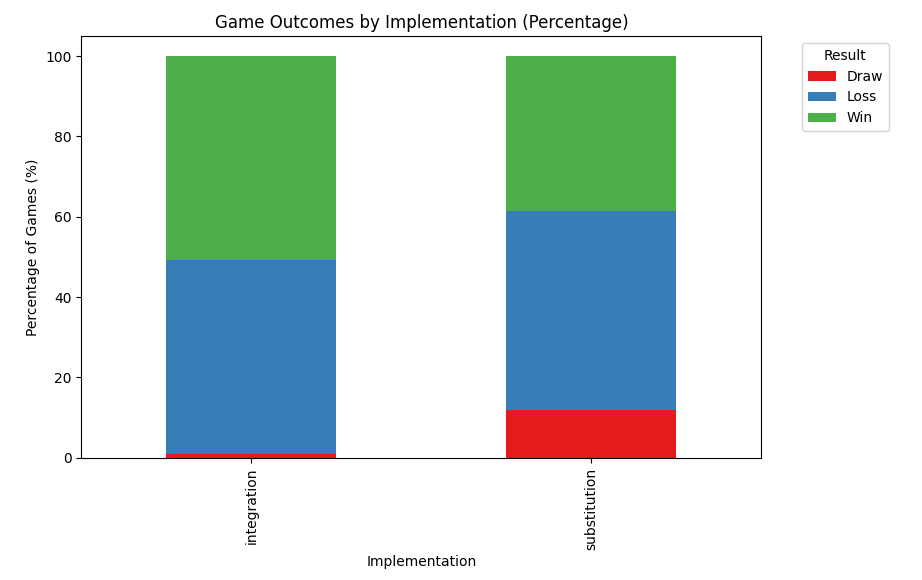
\includegraphics[width=0.8\textwidth]{images/plots/implementation/Implementation_vs_win_rate.png}
    \caption{Game Outcomes of each Implementation}
    \label{fig: implementation_vs_win_rate}
\end{figure}


% ======================================================================  
% OVERALL WIN/DRAW/LOSS RATES BY IMPLEMENTATION
% ======================================================================  
% integration (Total games: 8634):
%   Win:  4378 games (50.7%)
%   Draw: 84 games (1.0%)
%   Loss: 4172 games (48.3%)

% substitution (Total games: 3840):
%   Win:  1484 games (38.6%)
%   Draw: 460 games (12.0%)
%   Loss: 1896 games (49.4%)


% ======================================================================  
% WIN/DRAW/LOSS RATES BY IMPLEMENTATION AND OPPONENT
% ======================================================================  

% Opponent: random
% --------------------------------------------------
% integration (Total games: 4314):
%   Win:  4290 games (99.4%)
%   Draw: 24 games (0.6%)
%   Loss: 0 games (0%)

% substitution (Total games: 1920):
%   Win:  1484 games (77.3%)
%   Draw: 436 games (22.7%)
%   Loss: 0 games (0%)


% Opponent: stockfish
% --------------------------------------------------
% integration (Total games: 4320):
%   Win:  88 games (2.0%)
%   Draw: 60 games (1.4%)
%   Loss: 4172 games (96.6%)

% substitution (Total games: 1920):
%   Win:  0 games (0%)
%   Draw: 24 games (1.2%)
%   Loss: 1896 games (98.8%)


The integration implementation achieved a win rate of 50.7\%, with loses at 48.3\% and draws only at 1.0\%. In contrast, the substitution implementation achieved a win rate of 38.6\%, a similar loss rate of 49.4\% and a much higher draw rate of 12.0\%. This notable difference in draw rates suggests that MMNB substitution wasn't able to identify moves that would lead to wins even when in advantageous positions or the inability to identify crucial moves. 

It is important to seek deeper insight into this pattern by comparing the results of the two implementations against both opponents, Stockfish and random engine. Against the random opponent, MMNB integration dominated, winning 99.4\% of the games and never losing. MMNB substitution, however, did do well but achieved a much lower win rate of 77.3\% and a much higher draw rate of 22.7\%. This contrast of win rates, indicate that even against a low-skill opponent, with no strategy, the substitution engine was much worse at converting advantages into wins.

This is further supported by the games against Stockfish. MMNB integration was able to win 2.0\% of the games and draw 1.4\% of games whereas MMNB substitution failed to win even a single game, drawing only 1.2\% of the time and losing 98.8\% of the games. This highlights the limitation of the substitution implementation which is the evaluation function. The evaluation function which solely relies on the Naive Bayes probabilities, does not have the necessary understanding to win against a strong opponent. Despite being outperformed by Stockfish, the integration method showed that ability to exploit certain rare strategic opportunities, which is likely only due to the hybrid approach. These findings reinforce the hypothesis that Naive Bayes is best used as a supporting tool in a chess engine. The simplicity of the Naive Bayes classifier can provide some useful insights but is insufficient to be used as a standalone evaluation function.

Figure \ref{fig: implementation_vs_win_rate} is a good indicator of the overall performance of both engines but does not provide an insight of the quality of moves and efficiency of the engines. One way to measure the quality of moves is to compare the stockfish evaluation after each move as well as the average value of the blunders made by each engine. The results are shown in Figure \ref{fig: implementation_vs_stockfish_eval_and_blunder_value}.

\begin{figure}[H]
    \centering
    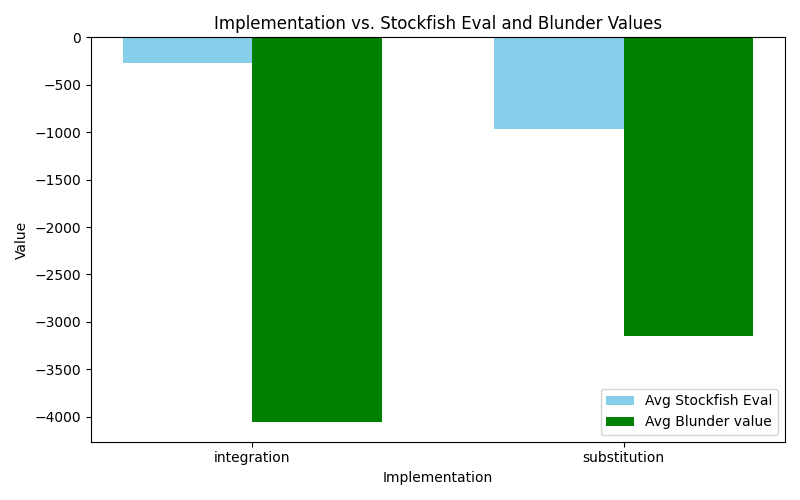
\includegraphics[width=0.8\textwidth]{images/plots/implementation/Implementation_vs_stockfish_eval_and_blunder_value.png}
    \caption{Stockfish Evaluation and Blunder Value of each Implementation}
    \label{fig: implementation_vs_stockfish_eval_and_blunder_value}
\end{figure}

% ======================================================================  
% AVERAGE STOCKFISH EVALUATION BY IMPLEMENTATION
% ======================================================================  
% integration: -340.02

%   By opponent:
%     vs random: 2241.98
%     vs stockfish: -2918.43

% substitution: -1048.25

%   By opponent:
%     vs random: 1099.23
%     vs stockfish: -3195.74

% ======================================================================
% AVERAGE BLUNDER SEVERITY BY IMPLEMENTATION (ONLY NON-ZERO BLUNDERS)
% ======================================================================
% integration: -4693.34 (13690 blunders)

%   By opponent:
%     vs random: -4617.38 (6200 blunders)
%     vs stockfish: -4756.22 (7490 blunders)

% substitution: -2652.59 (34364 blunders)

%   By opponent:
%     vs random: -2423.47 (30988 blunders)
%     vs stockfish: -4755.65 (3376 blunders)


The Stockfish evaluation is a numerical representation of the the move quality, where a higher value indicates a better move. Figure \ref{fig: implementation_vs_stockfish_eval_and_blunder_value} that the MMNB integration engine had a higher average stockfish evaluation than the MMNB substitution engine, which is consistent with the conclusions obtained based on the win rates. MMNB integration had an average stockfish evaluation of -340.02, whereas MMNB substitution had an average stockfish evaluation of -1048.25. However what is interesting is the average blunder value of each implementation. A blunder was defined as a move that caused a decrease in the Stockfish evalutaion by 300, where a more negative value indicates a more severe blunder based on Stockfish's opinion. MMNB integration had an average blunder value of -4693.34, whereas MMNB substitution had an average blunder value of -2652.59. This suggests that even though MMNB integration was able to win more games, it made more severe blunders. This could suggest that the integration method played much more aggressive and making more risky moves. This would explain the higher win rate but also the much higher average blunder value. Whereas the substitution engine played much more conservatively and avoided making more riskier moves, which is why it had a lower win rate since it was unable to exploit certain opportunities. 

% ======================================================================
% AVERAGE NUMBER OF NON-ZERO BLUNDERS PER WHOLE GAME BY IMPLEMENTATION
% ======================================================================
% integration (2160 games): 3.17 non-zero blunders per game

%   By opponent:
%     vs random (1080 games): 2.87 non-zero blunders per game
%     vs stockfish (1080 games): 3.47 non-zero blunders per game

% substitution (960 games): 17.90 non-zero blunders per game

%   By opponent:
%     vs random (480 games): 32.28 non-zero blunders per game
%     vs stockfish (480 games): 3.52 non-zero blunders per game

As much as blunder value indicates that integration caused much more severe blunders, it is also important to consider the average number of blunders made by each implementation. Despite the average blunder value being lower for the substitution implementation, it made over 6 times more blunders per game than the integration implementation. MMNB integration had an average of 3.17 blunders per game whereas MMNB substitution had an average of 17.90 blunders per game. This shows that the substitution implementation was much more prone to blunders, despite having a much lower average blunder value. This further 
confirms the theory that solely basing the evaluation function on the Naive Bayes classifier is detrimental to the engine's performance whereas a an approach that combines traditional methods and Naive Bayes can be much more fruitful.


Two good indicators of the performance of the engines during different phases of the game, is mobility and piece balance. Piece balance meaning the difference in material between both players and mobility referring to the number of possible moves the player can make. Figure \ref{fig: implementation_vs_avg_piece_balance_and_phase } and \ref{fig: implementation_vs_avg_mobility_and_phase} show the average piece balance and mobility of each implementation over different phases of the game. The opening phase was defined by the first 25\% of the game, midgame phase was defined by the next 50\% of the game and endgame was defined by the last 25\% of the game.

\begin{figure}[H]
    \centering
    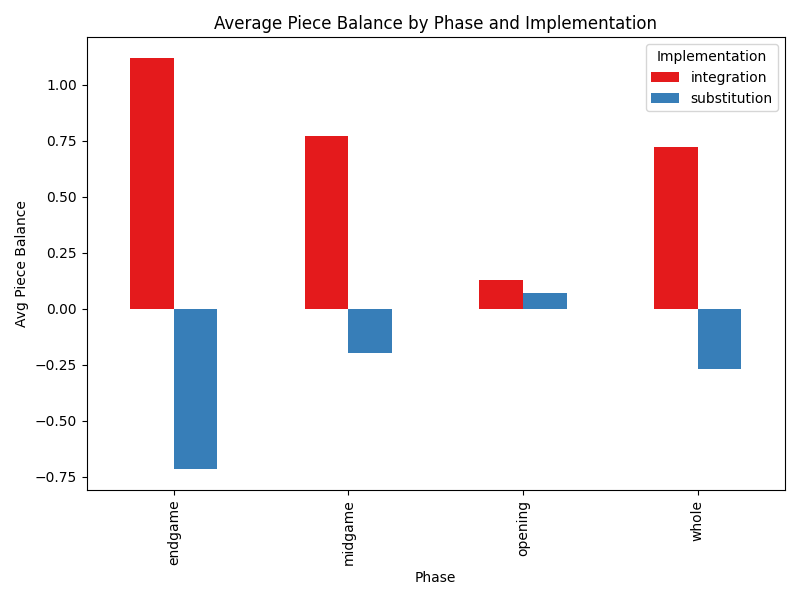
\includegraphics[width=0.8\textwidth]{images/plots/implementation/Implementation_vs_avg_piece_balance_and_phase.png}
    \caption{Average Piece Balance per Game of each Implementation}
    \label{fig: implementation_vs_avg_piece_balance_and_phase }
\end{figure}




% ======================================================================
% AVERAGE PIECE BALANCE BY PHASE AND IMPLEMENTATION  
% ======================================================================
% implementation  integration  substitution
% phase
% endgame            1.119188     -0.716872
% midgame            0.769215     -0.198002
% opening            0.126352      0.071598
% whole              0.722590     -0.267395

Figure \ref{fig: implementation_vs_avg_piece_balance_and_phase } shows that the integration method always had a higher piece balance than the substitution method across all the different game phases. MMNB integration achieved an average piece balance of 0.723, indicating the engine's understanding of the importance of having material advantage over the opponent. On the other hand, MMNB substitution has an average piece balance of -0.267, indicating that the engine was often at a material disadvantage. The integration implementation consistently outperformed the substitution implementation in piece balance across all game phases. Both implementations, in the opening phase, had similar positive piece balances indicating their understanding of the importance of material advantage. However during midgame and end game, MMNB integration considerably outperformed the substitution implementation, achieving an average piece balance of 0.769 and 1.119 respectively, whereas the substitution implementation had an average piece balance of -0.198 and -0.716 respectively. This highlights the integration method's ability to preserve and accumulate material advantage, across different stages. These observations suggest that combining Naive Bayes with a classical evaluation function supports better piece management and leads to fewer unfavourable trades. Conversely, reliance purely on Naive Bayes 
leads to more frequent disadvantageous exchanges, decreasing overall material count over time which is critical in the midgame and endgame phases. The hybrid approach evidently takes 
advantage of core chess principles, while still benefiting from probabilistic insights, resulting in higher piece balance and overall performance.

\begin{figure}[H]
    \centering
    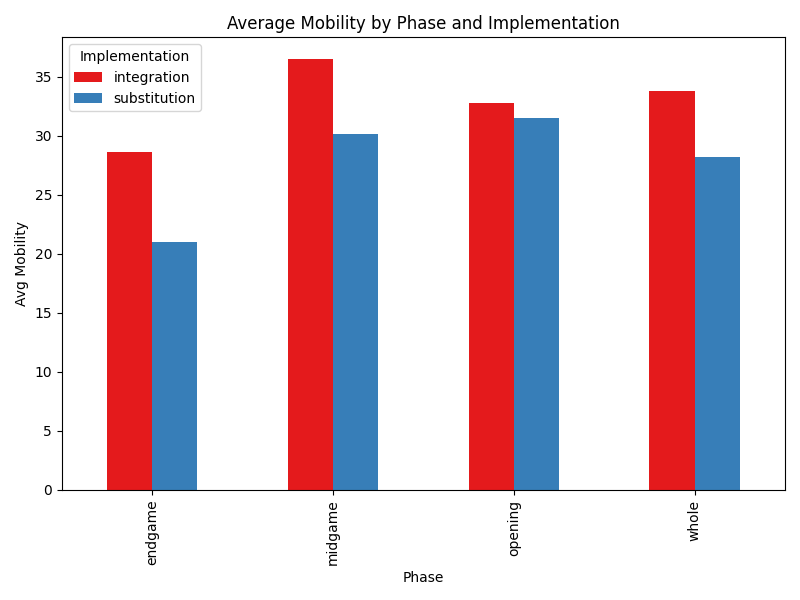
\includegraphics[width=0.8\textwidth]{images/plots/implementation/Implementation_vs_avg_mobility_and_phase.png}
    \caption{Average Mobility per Game of each Implementation}
    \label{fig: implementation_vs_avg_mobility_and_phase}
\end{figure}

% ======================================================================
% AVERAGE MOBILITY BY PHASE AND IMPLEMENTATION       
% ======================================================================
% implementation  integration  substitution
% phase
% endgame           28.583730     21.022493
% midgame           36.500683     30.159101
% opening           32.733946     31.481510
% whole             33.752626     28.199893


Mobility is measured by the average number of legal moves available at each turn. In chess theory, a higher mobility correlates with better board control, increasing tactical opportunities. Again, the integration method consistently surpassed the substitution method in mobility across all game phases. 
Overall, MMNB integration achieved an average mobility of 33.75 whereas MMNB substitution achieved an average mobility of 28.20, a gap of about 5.55 moves. In the opening, the average mobility is very similar inidicating similar strategies by both implementations. However, in midgame, where there is more complexity and opportunities since there are still a lot of pieces but are more developed. Integration has a higher mobility by about 6.34 moves (36.50 vs 30.16). This result was further amplified in the endgame where integration had an average mobility of 28.58 compared to 21.02 of the substitution implementation, a difference of 7.56 moves. Endgames require more precise and calculated moves minimising mistakes. This difference between the two indicates that MMNB substitution often causes pieces to move into more restricted or disadvantageous positions, while integration retains better piece coordination and mobility. There are a number of points that can be learnt from these results. Firstly, the integration method's superior mobility suggests it aims to avoid cramped locations and favour open positions, which is crucial throughout the game. MMNB substitution is strictly relying upon the assumption of feature independence. In the domain of chess where all features of the game are interdependent, it can lead to suboptimal decisions. The integration method's ability to combine the strengths of both Naive Bayes and traditional evaluation functions allows it to better navigate the complexities of chess, leading to improved mobility. These findings corroborate what has been concluded from previous metric results, indicating that pure Naive Bayes is less effective in understanding the nuances of the board while a hybrid approach preserves strategic principles and enhances mobility.

So far what has been assessed between the two implementations is different metrics to assess the performance of the engine. Another factor that is important to consider is the the time taken to make each move as if it is to be used in real time, it is important that it is able to make decisions in a reasonable time period. Figure \ref{fig: implementation_vs_avg_move_time_and_phase} shows the average time taken to make each move across the different phases of the game.

\begin{figure}[H]
    \centering
    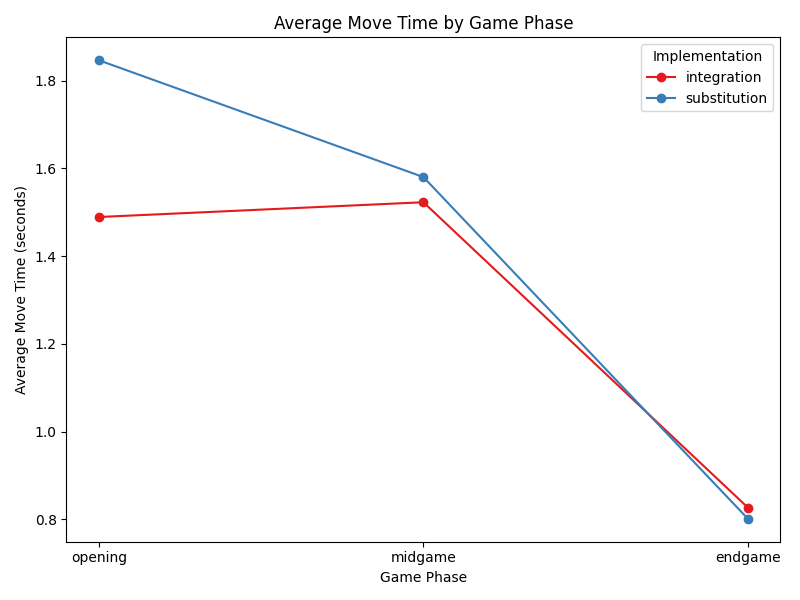
\includegraphics[width=0.8\textwidth]{images/plots/implementation/Implementation_vs_avg_move_time_and_phase.png}
    \caption{Average Time Taken to Make Each Move of each Implementation}
    \label{fig: implementation_vs_avg_move_time_and_phase}
\end{figure}

% Average Move Time by Phase and Implementation:
%      phase implementation  avg_move_times
% 0  opening    integration        1.489163
% 1  opening   substitution        1.846336
% 2  midgame    integration        1.522826
% 3  midgame   substitution        1.580211
% 4  endgame    integration        0.827023
% 5  endgame   substitution        0.801537
% 6    whole    integration        1.334166
% 7    whole   substitution        1.444066

The horizontal x-axis shows reflects the different phases of the game. The overall average time taken to make a move for MMNB integration was 1.334 seconds in comparison to 1.444 seconds for MMNB substitution. This indicates the integration method was able to make decisions faster than the substitution method. This is an important result as it hightlights that MMNB integration is not only more effective in winning games but also is more efficient in making decisions. In the opening phase, substitution has the longest move time at 1.846 seconds, which is 0.36 seconds longer than integration. This suggests that the pure Naive Bayes evaluation requires more computational effort or more likely, struggles to prune effectively early on. This is likely due to the fact that the opening phase there are many more pieces so a lot more possible moves, requiring more time to evaluate moves. In midgame the overall time taken to make a move decreases in both methods to 1.522 seconds for integration and 1.580 seconds for substitution. During the midgame phase, the complexity of the game increases however the overall number of pieces on the board decreases, which would require less time to evaluate moves. In the endgame phase, both engines drop below 1 second, with integration taking 0.827 seconds and substitution taking 0.801 seconds. This is expected as during endgame there are much less pieces on the board, reducing the branching factor of the search tree. Substitution is slightly faster than integration in the endgame phase,  but this is most likely due to what was discussed earlier and that substitution on average has less material on the board, resulting in less possible moves, requiring less time to evaluate. In the openinng and midgame phases, the substitution method seems to either take longer to evaluate moves or is less efficient in pruning the search tree. As the game progresses, there are less pieces and opportunities to make moves, narrowing the difference between the two implementations. Another important observation to note is the efficiency vs. effectiveness of the two implementations. Generally, an increase in one, causes a decrease in the other however the data shows otherwise. While substitution invests more time in evaluating moves, it is still not able to outperform integration, suggesting that longer computation time doesn't necessarily result in better moves. 

\begin{figure}[H]
    \centering
    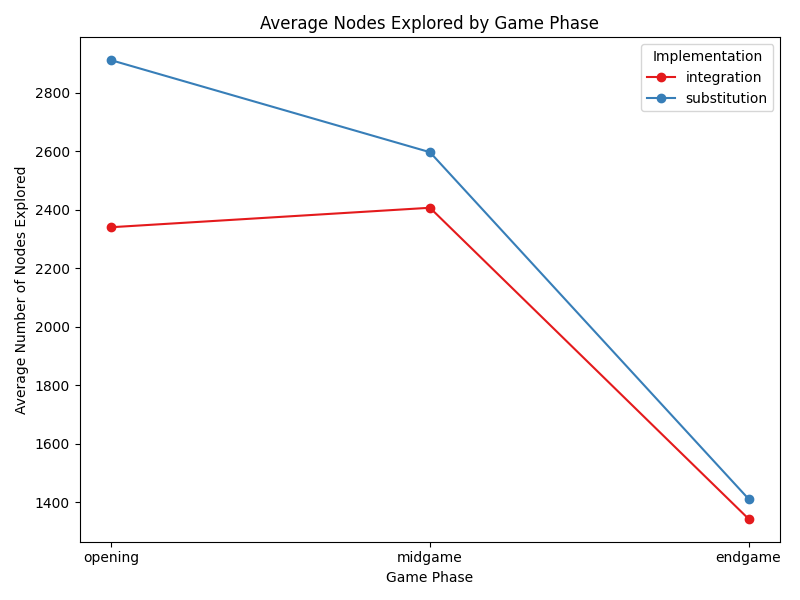
\includegraphics[width=0.8\textwidth]{images/plots/implementation/Implementation_vs_avg_nodes_explored_and_phase.png}
    \caption{Average Nodes Explored per Game of each Implementation}
    \label{fig: implementation_vs_avg_nodes_explored_and_phase}
\end{figure}

% Average Nodes Explored by Phase and Implementation:
%      phase implementation  avg_nodes_explored
% 0  opening    integration         2339.930400
% 1  opening   substitution         2910.269032
% 2  midgame    integration         2406.379927
% 3  midgame   substitution         2596.181826
% 4  endgame    integration         1343.829285
% 5  endgame   substitution         1411.950722
% 6    whole    integration         2114.515511
% 7    whole   substitution         2366.398302

Figure \ref{fig: implementation_vs_avg_nodes_explored_and_phase} shows the average number of nodes evaluated during the search of the game trees. The general trend is that the average number of nodes explored decreases as the game progresses. Similar to average time taken to make a move, this is expected as the number of pieces on the board decreases, reducing the branching factor of the search tree. The average number of nodes explored by MMNB integration was 2115 whereas the average number of nodes explored by MMNB substitution was 2366. In the opening phase, substitution explored 2910 nodes on average compared to 2339 for integration. This difference of 571 nodes indicates that the substitution method was less efficient in pruning the search tree, affirming the earlier observation that substitution takes longer to evaluate moves. The number of nodes explored closer to endgame is much closer between the two implementations. These results point towards the success of the hybrid approach in effectively pruning the search tree, leading to a more efficient evaluation process due ot the insight it gains from both the Naive Bayes classifier and the traditional evaluation function. 

These two figures show that MMNB substitution contiuously spends more time and searches more nodes in early phases of the game but despite this still fails to yield better results than MMNB integration. This pattern reinforces that combining Naive Bates with standard heuristics genreally results a more efficient and reliable approach to the minimax search over exclusively relying on Naive Bayes, particularly during opening phases.


\section{Feature Selection Analysis}

The feature sets were designed to be progressively more complex, with the aim of evaluating the impact of feature selection on the performance of the Naive Bayes classifier. The results from the previous section show that the addition of more features generally leads to better performance. However it is also important to see their impact on the gameplay of the engine. Figure \ref{fig: feature_set_vs_win_rate} shows the overall performance of each feature set in terms of wins, draws and losses.
\begin{figure}[H]
    \centering
    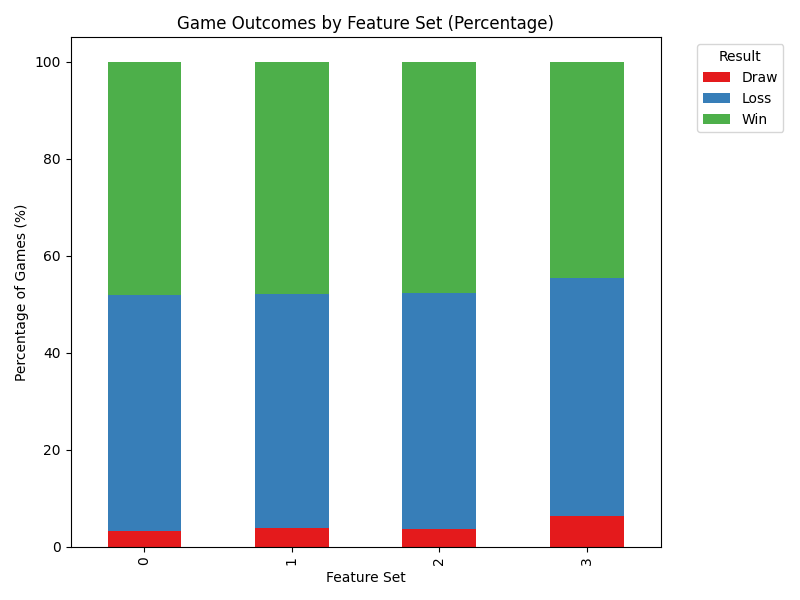
\includegraphics[width=0.8\textwidth]{images/plots/featureSet/Feature_set_vs_win_rate.png}
    \caption{Game Outcomes of each Feature Set}
    \label{fig: feature_set_vs_win_rate}
\end{figure}



% Feature Set 0:
%   Draw: 3.3%
%   Loss: 48.6%
%   Win: 48.1%
%   (Total games: 3360)

% Feature Set 1:
%   Draw: 3.9%
%   Loss: 48.2%
%   Win: 47.9%
%   (Total games: 2874)

% Feature Set 2:
%   Draw: 3.6%
%   Loss: 48.8%
%   Win: 47.6%
%   (Total games: 2880)

% Feature Set 3:
%   Draw: 6.4%
%   Loss: 49.0%
%   Win: 44.5%
%   (Total games: 3360)




Overall the different feature sets showed a similar trend in performance. Feature sets 0, 1 and 2 had win rates around 48\%, loss rates around 48\% to 49\% and draw raters around 3\% to 4\%. However, feature set 3 had a noticeable jump in draw rates to 6.4\%, nearly double the previous feature sets. It also had a noticeable decrease in win rates to 44.5\%. The increase in draw rates could suggest that the engine was more conservative in its play, staying away from riskier moves. This would also clarify the decrease in win rate since the engine was not able convert games into wins due to its defensive play. These results indicate that the addition of more features does not have a big impact on the gameplay of the engines. The similar win and loss rates across feature sets 0, 1 and 2 indicate the engine's ability to apply basic chess principles but was unable to apply the increasing complexity of the features and learn from the increased information. The sharp change in rates for feature set 3, however, indicate that the the complexity of the features may have caused the engine to become more uncertain in its moves, causing it to draw more and fail to win as much. This could be due to feature overlapping features causing the classifier to assign incorrect probabilities \cite{ahmedOkNBEnhancedOPTICS2024} or could indicate a possible overfitting of the model. These results also could show the diminishing results of adding more features. The more simpler features might have captured most of the information and the added specialised features did not increase the information gained by the model. One last point that is notable between the first 3 feature sets is that the loss rates were very similar, however there was a slight trend of decreasing win rates. Feature set 0 achieved a win rate of 48.1\%, feature set 1 achieved a win rate of 47.9\% and feature set 2 achieved a win rate of 47.6\%. This suggests that the adding of features didn't majorly affect the engine's vulnerability to losing but did add some confusion to the model, causing it to convert potential wins into draws. Overall, this data shows that adding features slightly changes teh results, it does not necessarily improve the winning ability of the engine, as would be expected. This is proven by feature set 3, which included the features of all the other feature sets and more, still had the lowest win rate and highest draw and loss rate. This indicates that the underlying assumption of feature independence in Naive Bayes struggles to handle the interactions between a large number of chess features. Thus concluding more features doe not necessarily translate to better performance but rather depends on the quality of features. 

Despite the similarity in win and loss rates, figures \ref{fig: feature_set_vs_piece_balance} and \ref{fig: feature_set_vs_blunder_count_and_avg_mobility} show different metrics of each feature set.

% ======================================================================
% METRICS BY FEATURE SET
% ======================================================================
% Feature Set 0:
%   Average Piece Balance: 0.475
%   Average Mobility: 31.699
%   Average Non-zero Blunders per Game: 7.258

% Feature Set 1:
%   Average Piece Balance: 0.464
%   Average Mobility: 32.574
%   Average Non-zero Blunders per Game: 6.957

% Feature Set 2:
%   Average Piece Balance: 0.552
%   Average Mobility: 32.324
%   Average Non-zero Blunders per Game: 6.728

% Feature Set 3:
%   Average Piece Balance: 0.207
%   Average Mobility: 31.695
%   Average Non-zero Blunders per Game: 9.615



\begin{figure}[H]
    \centering
    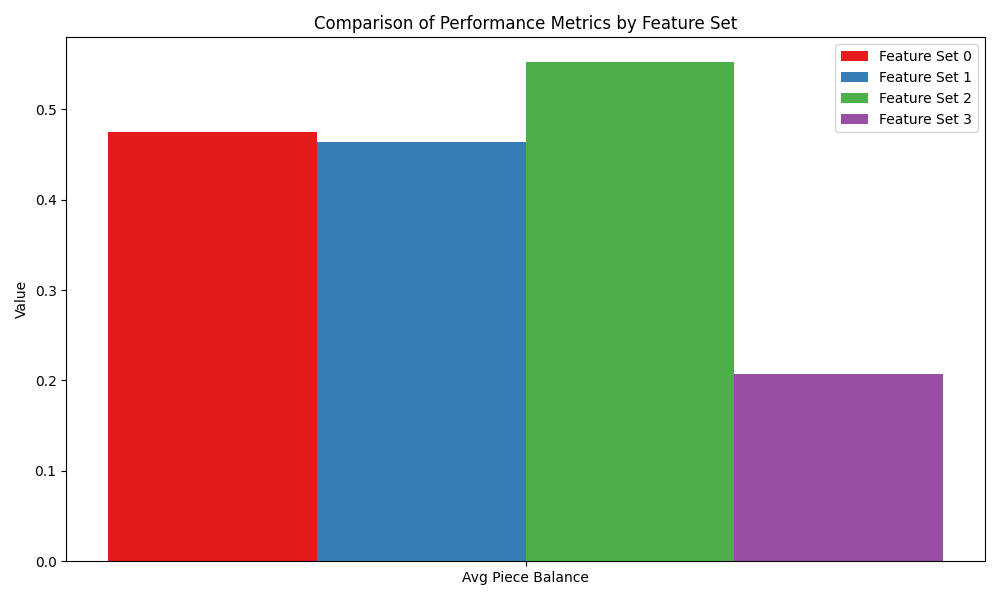
\includegraphics[width=0.8\textwidth]{images/plots/featureSet/Feature_set_vs_piece_balance.png}
    \caption{Average Piece Balance of each Feature Set}
    \label{fig: feature_set_vs_piece_balance}
\end{figure}


Figure \ref{fig: feature_set_vs_piece_balance} shows the average piece balance of each feature set. Overall, all feature sets had a positive piece balance, indicating the engine's strong understanding in the importance of material balance. All of the feature sets included material balance as a feature. Feature 2 stands out in the data, achieving an average piece balance of 0.552, 0.345 pieces higher than the lowest. Indicating its ability to retain more material or gain more material across the game. This feature set included pawn structure as a feature which proves the importance of pawn structure in chess and the impact it can have on the overall material balance of the game. Feature Set 3, surprisingly, again ranked the lowest with an average piece balance of 0.207. The additional complex features did not lead to improved material balance but rather made it significantly worse than the other feature sets. 


\begin{figure}[H]
    \centering
    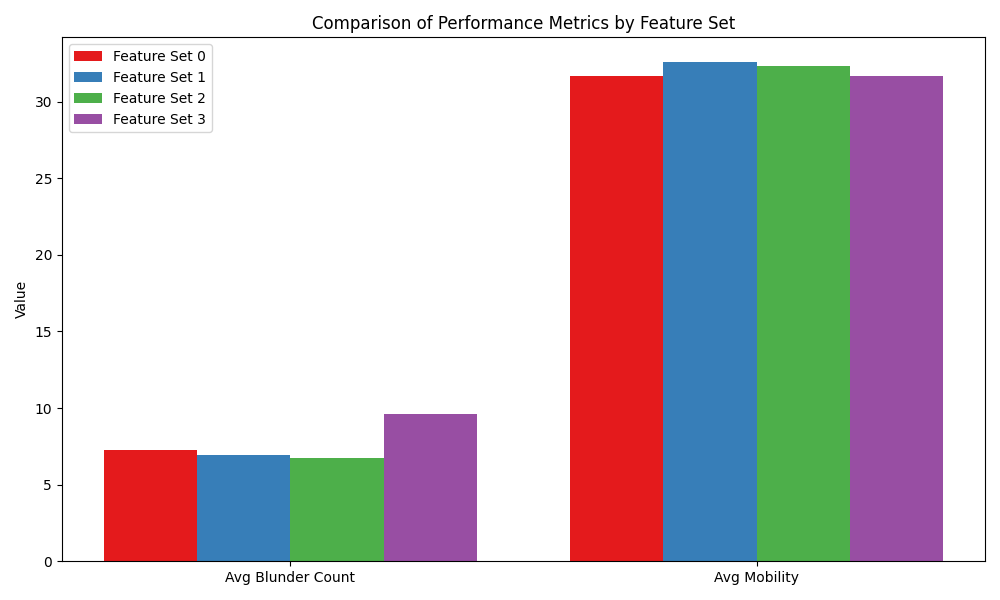
\includegraphics[width=0.8\textwidth]{images/plots/featureSet/Feature_set_vs_blunder_count_and_avg_mobility.png}
    \caption{Average Blunder Count and Mobility of each Feature Set}
    \label{fig: feature_set_vs_blunder_count_and_avg_mobility}
\end{figure}

Figure \ref{fig: feature_set_vs_blunder_count_and_avg_mobility} shows the average number of blunders made by each feature set per game. The general trend indicates the increase in features used, decreases the overall number of blunders made. Feature set 0 obtained a blunder count of 7.258, and feature set 2 achieved the  lowest at 6.728. This indicates the engine's increasingly ability to avoid making more blunders as more features were used, demonstrating the models increased learning. However, feature set 3 goes against this trend, obtaining the highest number of blunders per game at 9.615. Adding the most advanced features seem to unusually increase the number of severe mistakes made by the engine. This is provides further evidence that models trained using feature set suffer from overfitting or are affected by the dependency between features. The mobility of each feature set is roughly the same, with feature set 1 achieving the highest average mobility of 32.574 and feature set 0 achieving the lowest at 31.699. Higher mobility is a good indicator of better board control, resulting in more opportunities. 

Considering both graphs, it can be concluded that the feature set with the best overall performance is feature set 2. It achieved the highest piece balance, lowest blunder count and close to best mobility. It appears to be able to balance between complexity of features and model assumptions. The pawn structures introduced in this feature set, isolated and doubled pawns, add meaningful power without overcomplicating the model which could cause it to suffer. The most important point to understand from these results is the poor performance of feature set 3. Despite adding king safety, castling rights and game phase as features, it had the lowest piece balance, highest blunder count and close to bottom mobility. This suggests that the added features either caused the model to overfit or the fact that Naive Bayes fails to handle features that may contain more complex relationships. This demonstrates the importance of feature engineering, and that the increase in number of features does not necessarily lead to better performance but rather depends on the quality of features chosen. 


Finally, it is also important to analyse the efficiency of each feature set and if there is a benefit in using more complex features. Figures \ref{fig: feature_set_vs_avg_move_time} and \ref{fig: feature_set_vs_avg_nodes_explored} show the average time taken to make each move and the average number of nodes explored to decide each move.


% Average move times by feature set:
% Feature Set 0: 1.103 seconds
% Feature Set 1: 1.216 seconds
% Feature Set 2: 1.315 seconds
% Feature Set 3: 1.673 seconds

% Average nodes explored by feature set:
% Feature Set 0: 2225 nodes
% Feature Set 1: 2175 nodes
% Feature Set 2: 2143 nodes
% Feature Set 3: 2000 nodes


\begin{figure}[H]
    \centering
    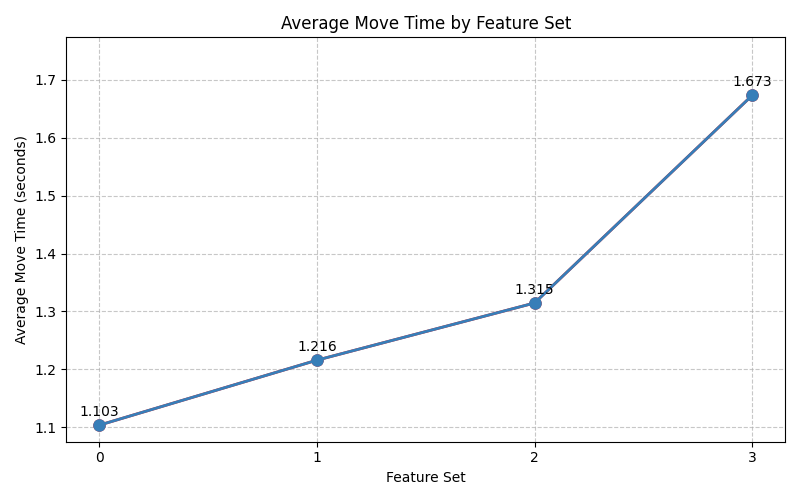
\includegraphics[width=0.8\textwidth]{images/plots/featureSet/Feature_set_vs_avg_move_time.png}
    \caption{Average Time Taken to Make Each Move of each Feature Set}
    \label{fig: feature_set_vs_avg_move_time} 
\end{figure}

Figure \ref{fig: feature_set_vs_avg_move_time} shows an overall trend of the increase in average time to make a move across the feature sets. It steadily increases from 1.103 seconds for feature set 0 to 1.315 seconds for feature set 2, which is as expected as more features are added, the model requires more time to calculate each feature, increasing the evaluation time. This is further supported by the sharp increase to 1.673 seconds for feature set 3. This is not only due to the increased number of features but also the drastic increase in the complexity of the features added. The addition of king safety, castling rights and game phase as features require much more computational effort to calculate. Even with a constant search depth, the evaluation becomes more expensive with increasing features. 


\begin{figure}[H]
    \centering
    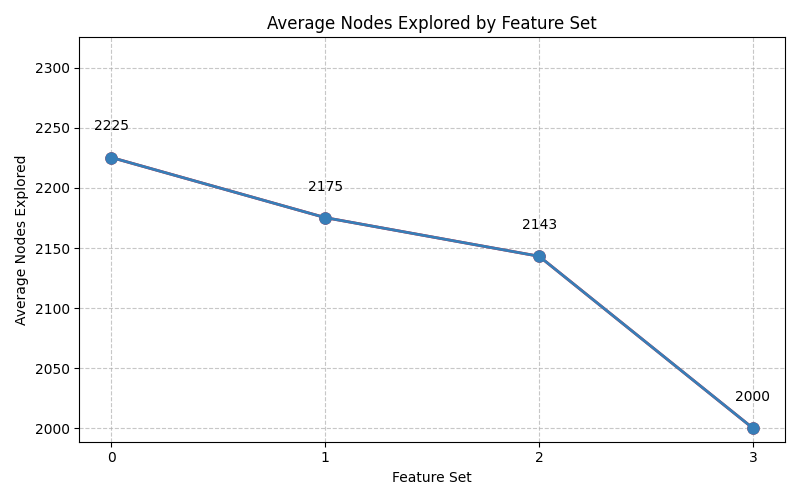
\includegraphics[width=0.8\textwidth]{images/plots/featureSet/Feature_set_vs_avg_nodes_explored.png}
    \caption{Average Nodes Explored per Game of each Feature Set}
    \label{fig: feature_set_vs_avg_nodes_explored}
\end{figure}

The general trend shown in figure \ref{fig: feature_set_vs_avg_nodes_explored} is that the average number of nodes explored decreases as the game progresses. There is a steady decrease between the first 3 feature sets from 2225 nodes for feature set 0 to 2143 nodes for feature set 2, with a more drastic decrease to 2000 nodes for feature set 3. This could suggest that the more complex features are able to prune the search tree more effectively. However, this goes against the earlier observation that the more complex features require more time to evaluate, since less nodes explored should lead to less time to decide a move. This suggests that the increase in time taken is not due to the number of nodes evaluated but rather the number of features used and the complexity of the features. 

What can be concluded from these results is that increasing the complexity of the features does  guarantee better outcomes. Despite fewer nodes being explored, the cost of evaluation increases the total move time significantly. In real-time chess engines, it is important to find a balance between a strong evaluation function and the efficiency of the evaluation. It also indicates the the additional overhead of utilising more features can be counterproductive.

\section{Dataset Analysis}

Another factor that may affect the performance of the engine is the dataset used to train the model. As mentioned before there were 3 datasets used to train the model. Master games, where one of the players had an Elo higher than 2200, beginner games, where both players had an Elo lower than 2200 and random games that took a random sample from the the whole dataset. Since there were only 300,000 master games in the dataset used, 300,000 games were also used for the beginner and random datasets. This was to ensure that the datasets were of similar size preventing any bias. Figure \ref{fig: dataset_vs_win_rate_pie} shows the outcomes of the games for each dataset.



% ======================================================================
% OVERALL WIN/DRAW/LOSS RATES BY DATASET    
% ======================================================================
% Dataset: master (Total games: 4318)       
%   Win:  2042 games (47.3%)
%   Draw: 180 games (4.2%)
%   Loss: 2096 games (48.5%)

% Dataset: random (Total games: 4318)       
%   Win:  2002 games (46.4%)
%   Draw: 212 games (4.9%)
%   Loss: 2104 games (48.7%)

% Dataset: beginner (Total games: 3838)     
%   Win:  1818 games (47.4%)
%   Draw: 152 games (4.0%)
%   Loss: 1868 games (48.7%)


% ======================================================================
% WIN/DRAW/LOSS RATES BY DATASET AND OPPONENT
% ======================================================================

% DATASET: master
% --------------------------------------------------
% Opponent: random (Total games: 2158)      
%   Win:  2014 games (93.3%)
%   Draw: 144 games (6.7%)
%   Loss: 0 games (0%)

% Opponent: stockfish (Total games: 2160)   
%   Win:  28 games (1.3%)
%   Draw: 36 games (1.7%)
%   Loss: 2096 games (97.0%)


% DATASET: random
% --------------------------------------------------
% Opponent: random (Total games: 2158)      
%   Win:  1966 games (91.1%)
%   Draw: 192 games (8.9%)
%   Loss: 0 games (0%)

% Opponent: stockfish (Total games: 2160)   
%   Win:  36 games (1.7%)
%   Draw: 20 games (0.9%)
%   Loss: 2104 games (97.4%)


% DATASET: beginner
% --------------------------------------------------
% Opponent: random (Total games: 1918)      
%   Win:  1794 games (93.5%)
%   Draw: 124 games (6.5%)
%   Loss: 0 games (0%)

% Opponent: stockfish (Total games: 1920)   
%   Win:  24 games (1.2%)
%   Draw: 28 games (1.5%)
%   Loss: 1868 games (97.3%)


\begin{figure}
    \centering
    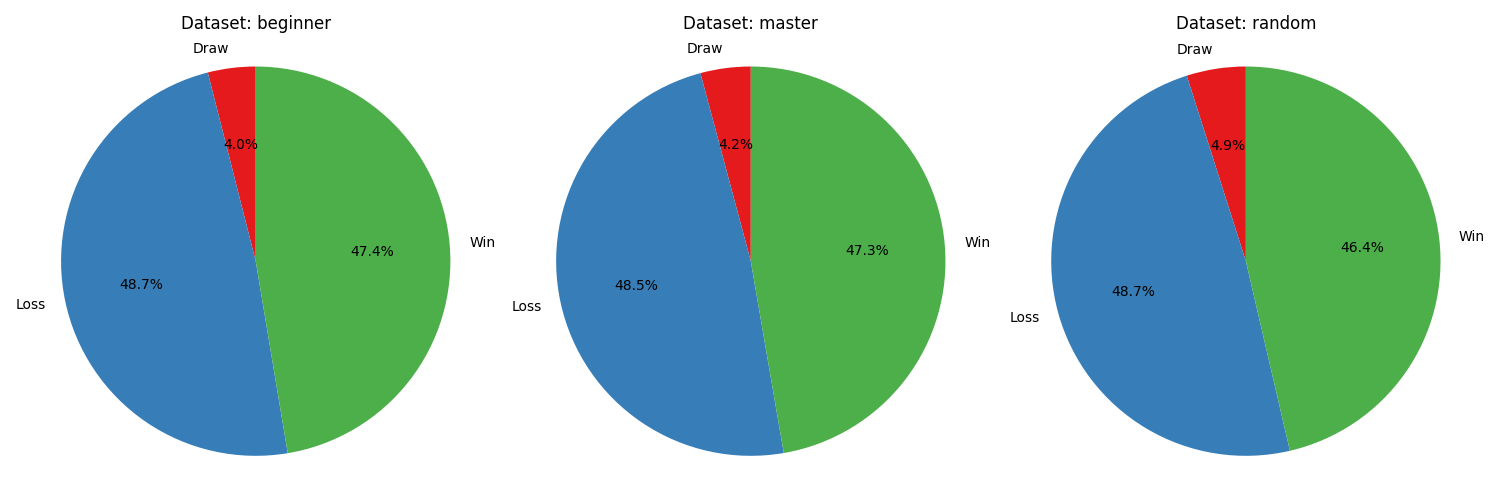
\includegraphics[width=0.8\textwidth]{images/plots/dataset/Dataset_vs_win_rate_pie.png}
    \caption{Win Rate of each Dataset}
    \label{fig: dataset_vs_win_rate_pie}
\end{figure}

The pie charts very minimal difference in performance across the three datasets. They all had win rates between 47\% and 48\%, loss rates between 48\% and 49\% and draw rates between 3\% and 4\%. This also indicates that the features used in the model have roughly equal power to identify winning and losing positions, regardless whether these positions came from a more experienced player or a less experienced player. This could be because the features used are very broad and are generally unaffected by the experience of the player, whereas other features may be more affected by the experience of the player. The most notable difference is the draw rate, where the random dataset had a draw rate of 4.9\% compared to 4.2\% for master and 4.0\% for beginner. This slight increase in the number of draws could be from mismatched skill levels or that the opponents used are not considered either master or beginner players. Due to the purpose of this project, the classifier only classified games into win or losses and did not utilise games that resulted in draws. This could explain the higher draw rate in the random dataset, since it was trained on a more diverse set of games. All three datasets won over 90\% of the games against random opponents, and losing no games against them. This domination by the engine confirms the ability of the engine to win from a position of strength. Against stockfish, all three datasets perform poorly obtaining an average loss rate of 97\% . What is interesting is that the the win rate of the random dataset against stockfish was slightly better than the other datasets, obtaining a win rate of 1.7\% compared to 1.3\% for master and 1.2\% for beginner. This could suggest the random dataset was able to generalise better to different positions and situations, due to the diverse games it used.

% ======================================================================
% BLUNDER ANALYSIS BY DATASET
% ======================================================================
% 1. AVERAGE NUMBER OF BLUNDERS PER GAME 
% --------------------------------------------------
% Dataset: master (1080 games): 7.92  blunders per game 

%   By opponent:
%     vs random (540 games): 12.49 blunders per game 
%     vs stockfish (540 games): 3.34 blunders per game 

% Dataset: random (1080 games): 8.21 blunders per game 

%   By opponent:
%     vs random (540 games): 12.89 blunders per game 
%     vs stockfish (540 games): 3.54 blunders per game 

% Dataset: beginner (960 games): 6.88 blunders per game 

%   By opponent:
%     vs random (480 games): 10.18 blunders per game 
%     vs stockfish (480 games): 3.58 blunders per game 


% 2. AVERAGE VALUE OF BLUNDERS      
% --------------------------------------------------
% Dataset: master: -3078.76 (8553 blunders)

%   By opponent:
%     vs random: -2624.54 (6747 blunders)
%     vs stockfish: -4775.67 (1806 blunders)

% Dataset: random: -3118.01 (8868 blunders)

%   By opponent:
%     vs random: -2661.88 (6959 blunders)
%     vs stockfish: -4780.77 (1909 blunders)

% Dataset: beginner: -3590.62 (6606 blunders)

%   By opponent:
%     vs random: -3197.91 (4888 blunders)
%     vs stockfish: -4707.93 (1718 blunders)


\begin{figure}
    \centering
    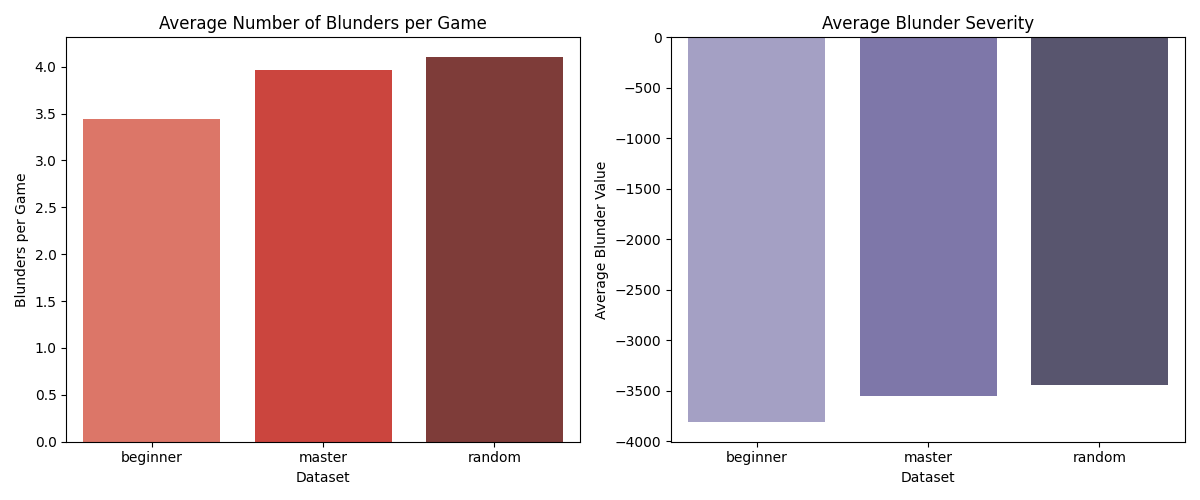
\includegraphics[width=0.8\textwidth]{images/plots/dataset/Dataset_vs_blunder_value_and_count.png}
    \caption{Average Blunder Value and Count of each Dataset}
    \label{fig: dataset_vs_blunder_value_and_count}
\end{figure}


Figure \ref{fig: dataset_vs_blunder_value_and_count} shows the number of blunders per game across each dataset and the average blunder value. Beginner has the lowest blunder count per game at around 3.34 blunders per game, while master and random have similar blunder counts of 3.54 and 3.58 respectively. Master level games generally include complex strategies and tactics which could have been misunderstood by the Naive Bayes classifier causing it to make more mistakes. Random data can also present more unpredicted situations, finding it difficult to differentiate whether it was a good move by a experienced player or a bad move from a less experienced player. However, the chart also shows that despite have a lower blunder count, the beginner dataset caused much worse blunders on average, with an average blunder value of -3590.62 compared to -3078.76 for master and -3118.01 for random. In beginner games, mistakes might directly lead to a large loss in material whereas master games may see more frequent blunders but less severe ones. This data indicates the importance of the training data in the performance of the engine and that there is a fine balance between the number of blunders and the severity of the blunders.


% ======================================================================
% AVERAGE PIECE BALANCE BY DATASET
% ======================================================================
% Dataset: master (1080 games): 0.419 average piece balance       

%   By opponent:
%     vs random (540 games): 1.670 average piece balance
%     vs stockfish (540 games): -0.831 average piece balance      

% Dataset: random (1080 games): 0.351 average piece balance       

%   By opponent:
%     vs random (540 games): 1.578 average piece balance
%     vs stockfish (540 games): -0.877 average piece balance      

% Dataset: beginner (960 games): 0.492 average piece balance      

%   By opponent:
%     vs random (480 games): 1.764 average piece balance
%     vs stockfish (480 games): -0.780 average piece balance 


\begin{figure}
    \centering
    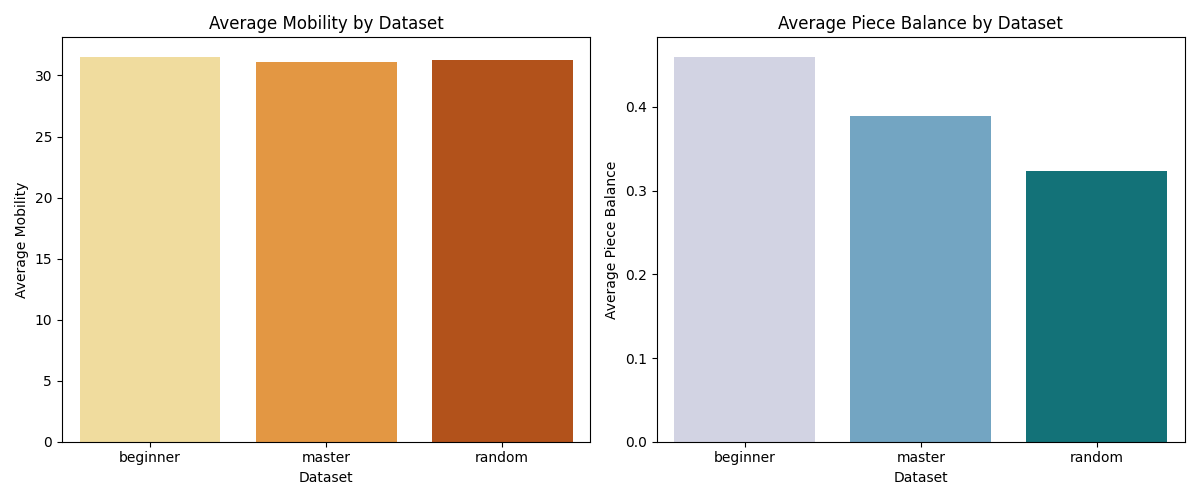
\includegraphics[width=0.8\textwidth]{images/plots/dataset/Dataset_vs_mobility_and_piece_balance.png}
    \caption{Average Mobility and Piece Balance of each Dataset}
    \label{fig: dataset_vs_mobility_and_piece_balance}
\end{figure}

Figure \ref{fig: dataset_vs_mobility_and_piece_balance} shows the average mobility and piece balance of each dataset. The mobility over all three dataset seems to be very similar showing a consistent understanding of the importance of mobility. However there was a big difference between the 3 datasets when it came to piece balance. The beginner dataset achieved the highest average piece balance of 0.492, while master and random achieved 0.419 and 0.351 respectively. This indicates that the beginner games the model was trained on, it learnt the importance of material advantage, which is a very basic principle most chess players acknowledge despite their level. The master dataset was also positive in its piece balance however was lower than the beginner dataset. This could be due to the complexity of the games and the strategies used by the players, which may have confused the model, especially not being able to understand long-term sacrifices that are common in master level games. The engine trained on the random elo data, achieved the lowest piece balance of 0.351. This could be due to the games it was trained on, it was not able to distinguish between strong and weak moves and patterns, causing it to make more unfavourable trades. 







\chapter{Legal, Social, Ethical and Professional Issues}
Your report should include a chapter with a reasoned discussion about legal, social ethical and professional issues within the context of your project problem. You should also demonstrate that you are aware of the regulations governing your project area and the Code of Conduct \& Code of Good Practice issued by the British Computer Society, and that you have applied their principles, where appropriate, as you carried out your project.

\section{Legal Issues}

As mentioned before, for this project the python-chess library was primarily used for the implementation of the chess engine. This library is licensed under the GNU General public License v3.0 (GPLv3) \cite{PythonchessPurePython}. This license is a free software license that allows developers to freely use, study and modify the python-chess library for their projects \cite{GNUGeneralPublic}. The license also requires that any modifications made to the library must be distributed under GPLv3, meaning that the source code mush be available to the public which is fulfilled as the source code is publicly available on GitHub \cite{fiekasNiklasfPythonchess2025}. 

This research utlises the `Chess' dataset available on Kaggle \cite{ChessGameDataset} uploaded by Mitchell J. The dataset is open to be used by the public under the Creative Commons CCO 1.0 Universal license, meaning that this dataset can be freely copied, modified, distributed and used for any purpose without requiring permission from the creator. Despite not legally required, we would like to acknowledge the contribution the creator has had on this research project and others. This data does not contain any directly identifiable information from Lichess users. Player usernames were included in the dataset but these do not directly reveal real-world identities. The data does not include sensitive personal data like real names, email addresses or phone numbers.

\section{Social Issues}

The chess engine developed in this project is a tool that can be used to help players improve their chess skills, however it has been engineered for someone who has some technical ability. Understanding python and basic command-line usage is required to run the engine. Also the output of the engine is standard algebraic notation which most chess players are familiar with, but players can not gain an understanding of why the engine made a particular move. A GUI was implemented to help users visualise the board and the moves made by the engine. This GUI would be more beneficial paired with a more readable explanation of the engine's moves. In the future, the engine could be more accessible to a wider audience by implementing features like audio outputs for visually impaired users or support for other languages. Another feature that could be beneficial is an Open API that would allow developers to integrate the engine into their own applications, potentially leading to more innovative ways to use the engine and more research opportunities. 

The advancements and increased accessibility of machine learning-based chess engines could have a major implications on the chess community. More powerful chess engines being very available could cause a reduction in demand for human chess coaches. These engines could provide personalised training, analyse moves and provide feedback to players, much better than a human coach may be able to do. This could lead to a decrease of people playing chess especially at the professional level. However this is very unlikely to replace human coaches but rather the increase in availability of chess engines could have a positive impact since it could allow those who may not have the resources to have a coach, lowering the barrier to entry for the game. It can be used as an educational tool for players, generating training exercises, analyse games and explain concepts.

\section{Ethical Issues}

An ethical advantage of using Naive Bayes over other machine learning techniques is its transparency and interpretability. Unlike models that are considered `black-boxes' like Neural Networks, Naive Byes allows users to understand the reasoning behind the model's predictions. Users are more likely to trust the model id they can understand the engine's thinking process. A Naive Bayes chess engine wouldn't necessarily harm a person's life, it is the responsibility of developers to consider the ethical implications it could have. One main risk is potential misuse of the engine, primarily in online gaming or competitions. For this reason, we encourage users to use the engine to use this tool for learning and analysis and strongly discourage any form of cheating and encourage fair play.

\section{Professional Issues}

This project was inline with the principles as mention in the Code of Conduct \& Code of Good Practice issued by the British Computer Society. I, Mohammad Ibrahim Khan, gave applied my knowledge and skills to the best of my ability and worked within my areas of competence and sought external guidance from my supervisor, Jeffery Raphael, where necessary. All data, results and conclusions presented in this report are accurate and truthful to the best of my knowledge. The intellectual property rights of others have been respected throughout, properly citing all external datasets, libraries and references. As discussed in previous sections, measures were taken to ensure privacy of individuals. Usernames were used as pseudonyms and no attempt was made to identify individuals.  

To ensure transparency and ease of use of the chess engine, a number of measures were taken

A number of measures were taken to ensure the transparency and ease of use of the chess engine. A detailed explanation of how the Naive Bayes classifier evaluates chess positions was provided in this report including the features used and the training process. The limitations of the engine such as potential bias and inability to understand complex situations have been clearly communicated as well as potential ethical issues related to the engine were also discussed. 
\chapter{Conclusion and Future Work}

The project's conclusions should list the key things that have been learnt as a consequence of engaging in your project work. For example, ``The use of overloading in C++ provides a very elegant mechanism for transparent parallelisation of sequential programs'', or ``The overheads of linear-time n-body algorithms makes them computationally less efficient than $O(n \log n)$ algorithms for systems with less than 100000 particles''. Avoid tedious personal reflections like ``I learned a lot about C++ programming...'', or ``Simulating colliding galaxies can be real fun...''. It is common to finish the report by listing ways in which the project can be taken further. This might, for example, be a plan for turning a piece of software or hardware into a marketable product, or a set of ideas for possibly turning your project into an MPhil or PhD.



???INCLUDE Training models on only a certain game phase like opening, mid or end

Also investigateing whcih features had the most impact, and if the complex features can be useful alone 

???

%%%%%%%%%%%%%%%%%%%%%%%%%%%%%%%%%
% References
%%%%%%%%%%%%%%%%%%%%%%%%%%%%%%%%%
\bibliographystyle{ieeetr}
\bibliography{references}
\addcontentsline{toc}{section}{Bibliography}


%%%%%%%%%%%%%%%%%%%%%%%%%%%%%%%%%
% Appendices
%%%%%%%%%%%%%%%%%%%%%%%%%%%%%%%%%
\appendix
% \include{Appendices/appendix}
\chapter{User Guide}

There are two main components of the codebase: one regarding the training of the model and one regarding the playing of chess games.

Before training, it is important to download the kaggle dataset from the link \url{https://www.kaggle.com/datasets/arevel/chess-games} and rename it to \texttt{chess\_games.csv}. It is also important to install all requierd libraries as listed in the \texttt{requirements.txt} file. The main files required for the training of the models are:

\begin{itemize}
    \item \texttt{dataset\_prep.py}: this is the main file to be executed to train the 12 models. This file loads the data, seperates the data into three groups, master level games, beginner level games and a random sample of games. For each combination of dataset and feature set, it preprocesses the data by invoking the \texttt{preprocess\_data} function from \texttt{data\_prep.py}. It then uses the processed data to train the model using the \texttt{train} function from \texttt{training.py}. It then saves the evaluation metrics to a CSV file.
    \item \texttt{data\_prep.py}: this file is used to preprocess the data and prepare it for training. It goes through each game in the dataset, simulates the games and extracts features are certain intervals. The \texttt{preprocess\_data} function returns the processed data, which is then used to train the model.
    \item \texttt{features.py}: contains all the methods to extract each feature. It also extracts features based on the feature set selected.
    \item \texttt{naive\_bayes.py}: This is the main file for the Naive Bayes model. It contains two main methods \texttt{predict} which returns the predicted class for a given set of features and \texttt{predict\_prob} which returns the probabilities for each class. 
    \item \texttt{training.py}: This file is where the main training occurrs. The data is first scaled use the the \texttt{prepare\_data} function. It then splits the data into training and testing data. It invokes the \texttt{fit} method from the \texttt{naive\_bayes.py} file to train the model. It then calculates a number of metrics such as accuracy, precision, recall, kaappa and F1 score and returns these metrics. It also saves the models and scalers to joblib files.
\end{itemize}


Before running the experiments, it is important to install stockfish ideally in the same directory as the \texttt{game.py} file. If it is not downloaded in the same directory, make sure to alter the \texttt{STOCKFISH\_PATH} in the \texttt{game.py} file to the path of the stockfish executable. It can be downloaded from the link \url{https://stockfishchess.org/download/}.
The main files require for the running of the experiments are:

\begin{itemize}
    \item \texttt{experiments.py}: this is the main file to be executed to run the experiments. It goes through all combinations of datasets, feature sets, naive bayes weightings, opponents and implementations and plays 30 games for each combination. It loads the models from the joblib files as well as the respective scalers. It calls the \texttt{play} function from the \texttt{game.py} file to play the games. It then saves the results to a CSV file.
    \item \texttt{game.py}: this is file where the game is played. In the \texttt{play} function, it keeps track of a number of metrics. It creates a new board and chooses a move by the engine base don the \texttt{get\_alphaBeta\_move} function, depending on the implementation selected. It then chooses a move either by a random engine or stockfish, depending on the opponent selected. It then continues this until the game is over. It then returns the different metrics of the game to be saved in a CSV file. 
    \item \texttt{minimax.py}: this file contains the \texttt{alphaBeta} function which implements a normal minimax algorithm with alpha beta pruning.
    \item \texttt{minimax\_NB\_integrated.py}: this file contains the \texttt{alphaBeta\_integrated} function which includes the implementation of the MMNB integration algorithm.
    \item \texttt{minimax\_NB\_sub.py}: this file contains the \texttt{alphaBeta\_sub} function which includes the implementation of the MMNB substitution algorithm.
\end{itemize}



% \section{Instructions}
% You must provide an adequate user guide for your software. The guide should provide easily understood instructions on how to use your software. A particularly useful approach is to treat the user guide as a walk-through of a typical session, or set of sessions, which collectively display all of the features of your package. Technical details of how the package works are rarely required. Keep the guide concise and simple. The extensive use of diagrams, illustrating the package in action, can often be particularly helpful. The user guide is sometimes included as a chapter in the main body of the report, but is often better included in an appendix to the main report.

% \chapter{Source Code}
\section{Instructions}
Complete source code listings must be submitted as an appendix to the report. The project source codes are usually spread out over several files/units. You should try to help the reader to navigate through your source code by providing a ``table of contents'' (titles of these files/units and one line descriptions). The first page of the program listings folder must contain the following statement certifying the work as your own: ``I verify that I am the sole author of the programs contained in this folder, except where explicitly stated to the contrary''. Your (typed) signature and the date should follow this statement.

All work on programs must stop once the code is submitted to KEATS. You are required to keep safely several copies of this version of the program and you must use one of these copies in the project examination. Your examiners may ask to see the last-modified dates of your program files, and may ask you to demonstrate that the program files you use in the project examination are identical to the program files you have uploaded to KEATS. Any attempt to demonstrate code that is not included in your submitted source listings is an attempt to cheat; any such attempt will be reported to the KCL Misconduct Committee.

\textbf{You may find it easier to firstly generate a PDF of your source code using a text editor and then merge it to the end of your report. There are many free tools available that allow you to merge PDF files.}





\end{document}
